\documentclass[11pt,a4paper]{article}

\usepackage[T1]{fontenc}
\usepackage[utf8]{inputenc}
\usepackage{lmodern}
\usepackage[margin=0.92in]{geometry}
\usepackage{amsmath,amssymb,amsthm,mathtools}
\usepackage{booktabs}
\usepackage{graphicx}
\usepackage{xcolor}
\usepackage{microtype}
\usepackage{enumitem}
\usepackage{hyperref}

\hypersetup{
  colorlinks=true,
  linkcolor=blue!65!black,
  citecolor=green!45!black,
  urlcolor=blue!65!black,
  pdftitle={Exact-Q Sum-of-Squares Hierarchy on the Normal Cone of Q2222},
  pdfauthor={Lluis Eriksson}
}

\newtheorem{theorem}{Theorem}[section]
\newtheorem{proposition}[theorem]{Proposition}
\newtheorem{corollary}[theorem]{Corollary}
\newtheorem{definition}[theorem]{Definition}
\newtheorem{remark}[theorem]{Remark}

\newcommand{\QQ}{\mathbb{Q}}
\newcommand{\RR}{\mathbb{R}}
\newcommand{\ZZ}{\mathbb{Z}}
\newcommand{\calQ}{\mathcal{Q}_{2222}}
\newcommand{\calL}{\mathcal{L}_{2222}}
\newcommand{\calN}{\mathcal{N}_{\mathcal{Q}}}
\newcommand{\calP}{\mathcal{P}}
\newcommand{\calB}{\mathcal{B}}
\newcommand{\calS}{\mathcal{S}}
\newcommand{\ext}{\operatorname{ext}}
\newcommand{\conv}{\operatorname{conv}}

\title{\textbf{Exact-$\QQ$ Sum-of-Squares Hierarchy on the Normal Cone of $\calQ$:\\
Rational Extreme-Point Parameterization, Four-Tier NPA Separation,\\
and Machine-Checked Visibility Optimality}}

\author{Lluis Eriksson\thanks{Independent researcher (Sweden). Prepared with AI assistance (Google Antigravity). Code, Lean~4 formalization, and exact-$\QQ$ certificates: \url{https://github.com/lluiseriksson/normal-cone-sos-hierarchy} (MIT license).}}

\date{November 2026}

\begin{document}
\maketitle

\begin{abstract}
Wu, Xie, and Ramanathan (\texttt{arXiv:2611.27413}, 2026) recently constructed the full three-dimensional normal cone $\calN(p^*)$ of Bell functionals uniquely maximized at every nonlocal extreme point $p^* \in \ext(\calQ)$ of the minimal $(2,2,2,2)$ quantum correlation set, enabling systematic optimization over all self-testing inequalities anchored to a fixed target behavior.
We resolve the algebraic, polyhedral, semidefinite-hierarchy, and noise-robustness structure of $\calN(p^*)$ in exact rational arithmetic over $\QQ$ and formalize all 20 foundational algebraic and soundness theorems in zero-dependency Lean~4 (\texttt{v4.35.0}, zero \texttt{sorry}, zero \texttt{Classical.choice}, zero warnings).
First, we introduce a dense rational parameterization $k \in \QQ \cap (1, 1+\sqrt{2})$ via $\alpha(k) = 2(1+2k-k^2)/(k^2+2k-1)$ and $\beta(k) = 4(k^2+1)/(k^2+2k-1)$ satisfying $\beta^2 = 8 + 2\alpha^2$ identically, rendering all eight coordinates of $p^*(k) \in \QQ^8$, the normal-cone basis $\{I_\alpha, S_\alpha, D_\alpha\}$, and every extreme ray of $\calN(p^*(k))$ strictly rational, while compressing the five-square Bamps--Pironio tilted-CHSH decomposition to a universal two-square identity $I_\alpha^2 + Q_\alpha^2 \equiv (8+2\alpha^2)I$.
Second, we prove that the cross-sectional polygon $\calP(k)$ of $\calN(p^*(k))$ undergoes an exact combinatorial octagon-to-hexagon phase transition governed by the cleared-denominator concurrency determinant $2(k^2+2k-1)^2(k^3-k^2-k-1)$, occurring precisely at the Tribonacci constant $k_{\mathrm{trib}} \approx 1.839287$.
Third, we uncover a sharp structural contrast inside the Navascu\'es--Pironio--Ac\'in (NPA) hierarchy on $\calN(p^*(k))$: restricting to the four-dimensional $N_3$-free annihilator subspace $\calS_4 = \operatorname{span}\{N_1, N_2, N_4, N_5\}$ collapses the sum-of-squares (SOS) cone onto the zero-area one-dimensional segment $\conv\{I_\alpha, \calB_{\mathrm{Bob}}(\alpha)\} = [-8\alpha/\beta^2, 0]\times\{0\}$, whereas restoring the fifth Level-$(1+AB)$ annihilator $N_3$ inflates $\mathcal{N}_{\mathrm{SOS}}^{(1+AB)}(p^*(2))$ into a curved two-dimensional spectrahedron covering $80.0\%$ of $\calP(2)$, nested strictly inside the NPA-2 spectrahedron $\mathcal{N}_{\mathrm{SOS}}^{(2)}(p^*(2))$ ($97.9\%$ area) and the true octagon $\calP(2)$.
Using an algebraic Level-1 annihilator proof ($\mathcal{N}_{\mathrm{SOS}}^{(1)}(p^*(k)) = \emptyset$ for all $k$) paired with exact rational $LDL^\top$ moment matrices and exact non-commutative SOS replays backed by weak SDP duality (Lean~4 Theorem~20), we establish the unconditional strict four-tier chain $\emptyset = \mathcal{N}_{\mathrm{SOS}}^{(1)}(p^*(2)) \subsetneq \mathcal{N}_{\mathrm{SOS}}^{(1+AB)}(p^*(2)) \subsetneq \mathcal{N}_{\mathrm{SOS}}^{(2)}(p^*(2)) \subsetneq \calN(p^*(2))$ with zero floating-point trust on every inclusion.
Fourth, we construct an explicit four-vertex rational linear-programming dual certificate proving that the canonical Alice-tilted CHSH functional $I_\alpha$ uniquely minimizes the white-noise visibility threshold $v(\calB) = \beta_{\mathrm{loc}}(\calB)/\beta_Q(\calB) \ge (2+\alpha)/\beta$ across the entire three-dimensional normal cone $\calN(p^*(k))$.
All results are backed by 13 standalone exact-$\QQ$ JSON certificates, four reproducible benchmarks, and a 42-attack adversarial red-team test suite.
\end{abstract}

\section{Introduction}
\label{sec:intro}

The convex body $\calQ \subset \RR^8$ of quantum behaviors in the minimal bipartite Bell scenario---two parties, two binary-outcome measurements per party---is the foundational arena of Bell nonlocality, device-independent (DI) randomness certification, and self-testing~\cite{chsh1969,tsirelson1980quantum,masanes2006asymptotic,acin2012randomness,yang2013robust,goh2018geometry,le2023quantum}.
Every nonlocal extreme point $p^* \in \ext(\calQ) \setminus \calL$ can be realized by projective measurements on a two-qubit pure state $|\psi_\theta\rangle = \cos\theta\,|00\rangle + \sin\theta\,|11\rangle$ and is uniquely exposed by the one-parameter family of tilted-CHSH Bell inequalities $I_\alpha$ ($\alpha \in (0,2)$) introduced by Ac\'in, Massar, and Pironio~\cite{acin2012randomness} and endowed with five-square sum-of-squares (SOS) self-testing decompositions by Bamps and Pironio~\cite{bamps2015sos}.

A landmark recent advance by Wu, Xie, and Ramanathan~\cite{wu2026normalcone} moved beyond single tilted-CHSH inequalities by explicitly characterizing the entire three-dimensional normal cone $\calN(p^*)$ of Bell functionals uniquely maximized at each nonlocal extreme behavior $p^* \in \ext(\calQ)$ and applying this cone to device-independent quantum information processing.
This breakthrough immediately raises four sharp mathematical and computational questions that govern how $\calN(p^*)$ behaves in practical DI certification and automated proof checking:
\begin{enumerate}[leftmargin=1.8em,itemsep=2pt]
  \item \emph{Exact rational arithmetic and minimal SOS rank:} Can $\ext(\calQ)$, its normal-cone basis, and its minimal SOS decompositions be parameterized densely over $\QQ$ without floating-point rounding or square-root irrationals, and can the Bamps--Pironio five-square SOS for $I_\alpha$ be compressed?
  \item \emph{Exact polyhedral combinatorics of $\calN(p^*)$:} How many extreme rays bound the two-dimensional cross-section $\calP(k)$ of $\calN(p^*(k))$ as the entanglement parameter varies across $(0,2)$, and where do combinatorial facet transitions occur?
  \item \emph{Exact NPA hierarchy certification power on $\calN(p^*)$:} Which Bell functionals inside the full three-dimensional normal cone admit exact Level-$(1+AB)$ or Level-2 NPA~\cite{npa2007bounding,npa2008convergent} sum-of-squares certificates of $\beta_Q(\calB) = \calB \cdot p^*$, what role does each exact annihilator play, and can every strict separation between Levels $1$, $1+AB$, $2$, and $\calN(p^*)$ be certified unconditionally over $\QQ$?
  \item \emph{Global white-noise robustness across $\calN(p^*)$:} Among all infinitely many Bell inequalities in $\calN(p^*)$ sharing the exact same unique quantum maximizer $p^*$, can any nontrivial normal-cone perturbation $(\eta,\zeta) \neq (0,0)$ beat the white-noise visibility threshold $v(I_\alpha) = (2+\alpha)/\sqrt{8+2\alpha^2}$ of the canonical tilted-CHSH inequality?
\end{enumerate}

In this paper we answer all four questions completely, with exact closed-form rational proofs, zero-floating-point-trust certificates, and a machine-checked Lean~4 kernel:
\begin{itemize}[leftmargin=1.5em,itemsep=2pt]
  \item \textbf{Rational Extreme-Point Atlas \& Universal 2-Square Identity (Theorem~\ref{thm:rational-2sq}):} Mapping $\alpha \mapsto \alpha(k) = 2(1+2k-k^2)/(k^2+2k-1)$ for $k \in \QQ \cap (1, 1+\sqrt{2})$ rationalizes $\beta(k) = \sqrt{8+2\alpha^2} = 4(k^2+1)/(k^2+2k-1) \in \QQ$ and places $p^*(k)$, $\{I_\alpha, S_\alpha, D_\alpha\}$, and all normal-cone vertices inside $\QQ$. In the universal involutive Bell algebra, $I_\alpha^2 + Q_\alpha^2 \equiv (8+2\alpha^2)I$ yields an exact two-square SOS certificate for $I_\alpha$ over $\QQ$.
  \item \textbf{Tribonacci Octagon-to-Hexagon Phase Transition (Theorem~\ref{thm:tribonacci}):} The cross-sectional polygon $\calP(k)$ switches sharply from an 8-vertex octagon ($k > k_{\mathrm{trib}}$) to a 6-vertex hexagon ($k < k_{\mathrm{trib}}$) precisely at the Tribonacci constant $k_{\mathrm{trib}} \approx 1.839286755$, the unique real root of $k^3 - k^2 - k - 1 = 0$, proved via an exact $3\times 3$ determinant factorization.
  \item \textbf{$\calS_4$-Subspace Collapse vs.\ Exact-$\QQ$ Four-Tier NPA Separation (Theorem~\ref{thm:hierarchy}):} Omitting the fifth Level-$(1+AB)$ annihilator $N_3$ collapses the SOS cone strictly onto the zero-area 1D segment $\conv\{I_\alpha, \calB_{\mathrm{Bob}}(\alpha)\} = [-8\alpha/\beta^2, 0]\times\{0\}$ (with exact 2-square rational SOS at both endpoints and closed-form Schur/diagonal obstructions outside). Restoring $N_3$ inflates $\mathcal{N}_{\mathrm{SOS}}^{(1+AB)}(p^*(2))$ to a 2D curved spectrahedron ($80.0\%$ of $\calP(2)$), nested strictly inside $\mathcal{N}_{\mathrm{SOS}}^{(2)}(p^*(2))$ ($97.9\%$) and $\calP(2)$. Every inclusion in $\emptyset = \mathcal{N}_{\mathrm{SOS}}^{(1)} \subsetneq \mathcal{N}_{\mathrm{SOS}}^{(1+AB)} \subsetneq \mathcal{N}_{\mathrm{SOS}}^{(2)} \subsetneq \calN(p^*(2))$ is proved in exact $\QQ$ via mutually exclusive SOS replays and strictly positive-definite $LDL^\top$ NPA moment matrices.
  \item \textbf{Unique Global White-Noise Visibility Optimality (Theorem~\ref{thm:visibility}):} An explicit strictly positive four-vertex rational LP dual certificate proves $v(\calB(\eta,\zeta)) \ge (2+\alpha)/\beta$ throughout $\calN(p^*(k))$, with equality uniquely at $(\eta,\zeta) = (0,0)$.
  \item \textbf{Zero-Trust Formal Verification:} All 20 core algebraic and weak-SDP-duality soundness theorems are machine-checked in Lean~4 (\texttt{v4.35.0}, zero \texttt{sorry}, zero \texttt{Classical.choice}, zero warnings); 13 standalone exact-$\QQ$ JSON certificates spanning all four weak-SDP-duality-sound modes are independently replayed in pure Python stdlib (\texttt{fractions.Fraction}); and a 42-attack adversarial red-team test suite validates certificate tamper resistance.
\end{itemize}

\section{Preliminaries and Exact Normal-Cone Coordinates}
\label{sec:prelim}

We work in the standard eight-dimensional Collins--Gisin / correlator representation of no-signaling $(2,2,2,2)$ behaviors:
\begin{equation}
  p = \bigl(\langle A_0\rangle,\; \langle A_1\rangle,\; \langle B_0\rangle,\; \langle B_1\rangle,\; \langle A_0 B_0\rangle,\; \langle A_0 B_1\rangle,\; \langle A_1 B_0\rangle,\; \langle A_1 B_1\rangle\bigr) \in [-1,1]^8,
\end{equation}
where $A_x, B_y$ are Hermitian involutions ($A_x^2 = B_y^2 = I$) satisfying $[A_x, B_y] = 0$ for $x,y \in \{0,1\}$.
The local polytope $\calL = \conv\{v(a_0,a_1,b_0,b_1) : a_x, b_y \in \{-1,+1\}\}$ has 16 deterministic extreme points $v(a_0,a_1,b_0,b_1) = (a_0, a_1, b_0, b_1, a_0 b_0, a_0 b_1, a_1 b_0, a_1 b_1)$.
For any Bell functional $\calB \in \RR^8$, its local bound is $\beta_{\mathrm{loc}}(\calB) = \max_{v \in \ext(\calL)} \calB \cdot v$, its quantum bound is $\beta_Q(\calB) = \sup_{p \in \calQ} \calB \cdot p$, and for any Bell-violating functional ($\beta_Q(\calB) > \beta_{\mathrm{loc}}(\calB) > 0$) its white-noise visibility threshold is
\begin{equation}
  v(\calB) := \inf\bigl\{v \in [0,1] : v\, p^* + (1-v)\, p_{\mathrm{noise}} \text{ violates } \calB \cdot p \le \beta_{\mathrm{loc}}(\calB)\bigr\} = \frac{\beta_{\mathrm{loc}}(\calB)}{\beta_Q(\calB)},
\end{equation}
since the isotropic white-noise behavior is $p_{\mathrm{noise}} = (0,0,0,0,0,0,0,0) \in \RR^8$.

Following Ac\'in--Massar--Pironio~\cite{acin2012randomness} and Bamps--Pironio~\cite{bamps2015sos}, the canonical tilted-CHSH operator for $\alpha \in (0,2)$ is
\begin{equation}
  I_\alpha = \alpha A_0 + A_0(B_0 + B_1) + A_1(B_0 - B_1),
\end{equation}
represented by the coordinate vector $I_\alpha = (\alpha, 0, 0, 0, 1, 1, 1, -1) \in \RR^8$, with local bound $\beta_{\mathrm{loc}}(I_\alpha) = 2 + \alpha$ and quantum bound $\beta := \beta_Q(I_\alpha) = \sqrt{8 + 2\alpha^2}$.
Up to local symmetries, the unique quantum behavior achieving $I_\alpha \cdot p^* = \beta$ is realized by the two-qubit state $|\psi_\theta\rangle = \cos\theta\,|00\rangle + \sin\theta\,|11\rangle$ with $\sin(2\theta) = \sqrt{(4-\alpha^2)/(4+\alpha^2)}$ and projective measurements $A_0 = \sigma_z$, $A_1 = \sigma_x$, $B_0 = \cos\mu\,\sigma_z + \sin\mu\,\sigma_x$, $B_1 = \cos\mu\,\sigma_z - \sin\mu\,\sigma_x$ where $\tan\mu = \sin(2\theta)$~\cite{bamps2015sos,wu2026normalcone}.
Evaluating the eight correlators yields the exact algebraic form
\begin{equation}
  p^*(\alpha) = \left(\frac{2\alpha}{\beta},\; 0,\; \frac{\alpha}{2},\; \frac{\alpha}{2},\; \frac{\beta}{4},\; \frac{\beta}{4},\; \frac{4-\alpha^2}{2\beta},\; -\frac{4-\alpha^2}{2\beta}\right),
  \label{eq:pstar}
\end{equation}
which satisfies $I_\alpha \cdot p^*(\alpha) = \frac{2\alpha^2}{\beta} + \frac{\beta}{2} + \frac{4-\alpha^2}{\beta} = \frac{8+2\alpha^2}{2\beta} + \frac{\beta}{2} = \beta$.

By the first-order stationarity construction of Wu, Xie, and Ramanathan~\cite{wu2026normalcone}, every Bell functional $\calB \in \RR^8$ that is stationary at $p^*(\alpha)$ on the smooth five-dimensional manifold of nonlocal extreme behaviors $\ext(\calQ)$ lies in a three-dimensional linear subspace spanned by $I_\alpha$ together with two exact tangent-orthogonal generators:
\begin{align}
  S_\alpha &= \left(\frac{\beta^2}{8},\; 0,\; -\frac{\beta}{4},\; -\frac{\beta}{4},\; \frac{\alpha}{2},\; \frac{\alpha}{2},\; 0,\; 0\right), \label{eq:Salpha}\\
  D_\alpha &= \left(0,\; -\frac{\beta^2}{8},\; \frac{\beta}{4},\; -\frac{\beta}{4},\; 0,\; 0,\; \frac{\alpha}{2},\; \frac{\alpha}{2}\right). \label{eq:Dalpha}
\end{align}
One checks directly from~\eqref{eq:pstar}--\eqref{eq:Dalpha} that
\begin{equation}
  S_\alpha \cdot p^*(\alpha) = \frac{\alpha\beta}{4}, \qquad D_\alpha \cdot p^*(\alpha) = 0.
\end{equation}
Normalizing the coefficient of $I_\alpha$ to $1$, we parameterize the two-dimensional cross-section of $\calN(p^*(\alpha))$ by
\begin{equation}
  \calB(\eta,\zeta) := I_\alpha + \eta S_\alpha + \zeta D_\alpha, \qquad \beta_Q(\calB(\eta,\zeta)) = \beta + \frac{\alpha\beta}{4}\,\eta.
  \label{eq:B-etazeta}
\end{equation}
As proved in~\cite{wu2026normalcone}, for the $\calQ$ boundary the 16 local-vertex dominance inequalities $\calB(\eta,\zeta) \cdot v \le \calB(\eta,\zeta) \cdot p^*(\alpha)$ ($v \in \ext(\calL)$) carve out the exact two-dimensional convex polygon $\calP(\alpha)$ of Bell functionals uniquely exposing $p^*(\alpha)$ (with strict interior $\beta_{\mathrm{loc}} < \beta_Q$ and boundary edges $\beta_{\mathrm{loc}} = \beta_Q$).

\section{Main Theorems}
\label{sec:theorems}

\subsection{Dense Rational Parameterization and Universal Two-Square SOS}

\begin{theorem}[Rational Extreme-Point Atlas and Universal 2-Square {$\ZZ[\alpha]$} Identity]
\label{thm:rational-2sq}
Let $k \in \QQ \cap (1, 1 + \sqrt{2})$ and define $D(k) := k^2 + 2k - 1 > 0$,
\begin{equation}
  \alpha(k) := \frac{2(1 + 2k - k^2)}{k^2 + 2k - 1}, \qquad \beta(k) := \frac{4(k^2 + 1)}{k^2 + 2k - 1}.
  \label{eq:rational-param}
\end{equation}
Then:
\begin{enumerate}[leftmargin=1.8em,itemsep=2pt]
  \item $\alpha(k) \in \QQ \cap (0,2)$ is strictly decreasing and maps $\QQ \cap (1, 1+\sqrt{2})$ onto a dense subset of $(0,2)$, while $\beta(k)^2 = 8 + 2\alpha(k)^2$ holds identically.
  \item All eight coordinates of $p^*(k) \in \ext(\calQ)$, all entries of $I_\alpha, S_\alpha, D_\alpha$, and all extreme rays of the normal cone $\calN(p^*(k))$ belong strictly to $\QQ$.
  \item In the involutive algebra $A_x^2 = B_y^2 = I$, $[A_x, B_y] = 0$, defining $Q_\alpha := -\alpha A_1 + A_1(B_0 + B_1) + A_0(B_0 - B_1)$, the exact polynomial identity
  \begin{equation}
    I_\alpha^2 + Q_\alpha^2 \equiv (8 + 2\alpha^2)\, I
    \label{eq:two-square-id}
  \end{equation}
  holds over $\ZZ[\alpha]$. Consequently, for every $k \in \QQ \cap (1, 1+\sqrt{2})$, the shifted Bell operator admits an exact rank-$2$ rational sum-of-squares certificate
  \begin{equation}
    \beta(k)\, I - I_{\alpha(k)} = \frac{1}{2\beta(k)}\bigl(\beta(k)\, I - I_{\alpha(k)}\bigr)^2 + \frac{1}{2\beta(k)}\, Q_{\alpha(k)}^2.
    \label{eq:two-square-sos}
  \end{equation}
\end{enumerate}
\end{theorem}

\begin{proof}
Direct algebraic expansion yields
\begin{equation}
  \bigl(4(k^2+1)\bigr)^2 = 16(k^4 + 2k^2 + 1) = 8(k^2 + 2k - 1)^2 + 2\bigl(2(1 + 2k - k^2)\bigr)^2,
\end{equation}
machine-checked over $\ZZ$ as \texttt{NormalConeSOS.pythagorean\_tilted\_identity}.
On $k \in (1, 1+\sqrt{2})$, both $k^2+2k-1 > 2$ and $1+2k-k^2 = 2-(k-1)^2 \in (0,2)$ are strictly positive, and $2(1+2k-k^2) < 2(k^2+2k-1) \iff k^2 > 1$, so $\alpha(k) \in (0,2)$; rationality of $p^*(k)$, $\{I_\alpha, S_\alpha, D_\alpha\}$, and all intersections of rational half-spaces follows immediately.
For~\eqref{eq:two-square-id}, writing $C_+ := B_0 + B_1$ and $C_- := B_0 - B_1$, note that $C_+^2 + C_-^2 = 4I$ and $C_+ C_- + C_- C_+ = 0$. Expanding $I_\alpha^2$ and $Q_\alpha^2$ gives
\begin{align}
  I_\alpha^2 &= \alpha^2 I + C_+^2 + C_-^2 + 2\alpha C_+ + \alpha\{A_0, A_1\} C_- + [A_0, A_1] C_+ C_-,\\
  Q_\alpha^2 &= \alpha^2 I + C_+^2 + C_-^2 - 2\alpha C_+ - \alpha\{A_0, A_1\} C_- - [A_0, A_1] C_+ C_-,
\end{align}
where $C_+ C_- = -C_- C_+ = [B_0, B_1]$. Every cross-term cancels identically, leaving $I_\alpha^2 + Q_\alpha^2 = 2\alpha^2 I + 2(C_+^2 + C_-^2) = (8 + 2\alpha^2)I = \beta^2 I$. Rearranging $(\beta I - I_\alpha)^2 + Q_\alpha^2 = 2\beta(\beta I - I_\alpha)$ gives~\eqref{eq:two-square-sos} (Lean~4: \texttt{two\_square\_sos\_identity}).
\end{proof}

\begin{remark}
Bamps and Pironio~\cite{bamps2015sos} construct a five-square SOS decomposition for $\beta I - I_\alpha$ to extract algebraic self-testing relations directly. Theorem~\ref{thm:rational-2sq} shows that for certifying the exact quantum bound $\beta_Q(I_\alpha) = \beta$ itself, only \emph{two} squares suffice, and both lie in the nine-operator Level-$(1+AB)$ basis with purely rational coefficients over $\QQ$.
\end{remark}

\subsection{Exact Normal-Cone Polygon and Tribonacci Phase Transition}

\begin{theorem}[Tribonacci Octagon-to-Hexagon Phase Transition of $\calN(p^*(k))$]
\label{thm:tribonacci}
Let $k \in (1, 1+\sqrt{2})$ with $D = k^2 + 2k - 1 > 0$, and consider the 16 local-vertex half-spaces
\begin{equation}
  L_{a_0,a_1,b_0,b_1}(\eta,\zeta) := \calB(\eta,\zeta)\cdot v(a_0,a_1,b_0,b_1) - \calB(\eta,\zeta)\cdot p^*(k) \le 0
\end{equation}
defining the normal-cone cross-section $\calP(k) \subset \RR^2$.
After clearing strictly positive denominators, the three upper-half-plane facet linear forms $L_{(-1,-1,-1,-1)}$, $L_{(1,1,1,-1)}$, and $L_{(1,-1,1,1)}$ have exact integer coefficient matrix
\begin{equation}
  M(k) = \begin{pmatrix}
    -D & k^2 - 1 & 2k^2 \\
    -(k-1)D & k(k^2 + 1) & k^2 + 1 \\
    -D & -2k & (k+1)^2
  \end{pmatrix},
\end{equation}
whose determinant factors identically over $\ZZ[k]$ as
\begin{equation}
  \det M(k) = 2 D^2 \bigl(k^3 - k^2 - k - 1\bigr).
  \label{eq:tribonacci-det}
\end{equation}
By $\zeta \mapsto -\zeta$ symmetry, the reflected triple $L_{(-1,1,-1,-1)}$, $L_{(1,-1,-1,1)}$, $L_{(1,1,1,1)}$ satisfies the identical factorization up to sign. Consequently, $\calP(k)$ undergoes an exact combinatorial phase transition at the Tribonacci constant $k_{\mathrm{trib}} \approx 1.839286755214$ ($\alpha_{\mathrm{trib}} \approx 0.427480726$), the unique real root of $k^3 - k^2 - k - 1 = 0$:
\begin{itemize}[leftmargin=1.5em,itemsep=1pt]
  \item For $k \in (k_{\mathrm{trib}}, 1+\sqrt{2})$ ($\alpha < \alpha_{\mathrm{trib}}$), $\calP(k)$ is a strictly convex \textbf{8-vertex octagon} bounded by the four upper facets $F_1 = L_{(1,1,1,-1)}$, $F_2 = L_{(-1,-1,-1,-1)}$, $F_3 = L_{(1,-1,1,1)}$, $F_4 = L_{(-1,1,1,-1)}$ and their four $\zeta \mapsto -\zeta$ reflections.
  \item For $k \in (1, k_{\mathrm{trib}})$ ($\alpha > \alpha_{\mathrm{trib}}$), the antipodal facets $F_2 = L_{(-1,-1,-1,-1)}$ and $F_2' = L_{(-1,1,-1,-1)}$ become strictly redundant and $\calP(k)$ is a strictly convex \textbf{6-vertex hexagon} bounded by $\{F_1, F_3, F_4\}$ and their reflections; at the exact transition point $k = k_{\mathrm{trib}}$, $F_2$ and $F_2'$ pass through the vertices $F_1 \cap F_3$ and $F_1' \cap F_3'$ (triple concurrency), so $\calP(k_{\mathrm{trib}})$ is also a 6-vertex hexagon.
\end{itemize}
\end{theorem}

\begin{proof}
Substituting~\eqref{eq:rational-param} into $L_{a_0,a_1,b_0,b_1}(\eta,\zeta) = c_0 + c_1 \eta + c_2 \zeta$ for the four upper-half-plane candidate facets $F_1 = L_{(1,1,1,-1)}$, $F_2 = L_{(-1,-1,-1,-1)}$, $F_3 = L_{(1,-1,1,1)}$, and $F_4 = L_{(-1,1,1,-1)}$ yields
\begin{align}
  F_1 &= \frac{4(k-1)}{D^2}\bigl(-(k-1)D + k(k^2+1)\eta + (k^2+1)\zeta\bigr),\\
  F_2 &= \frac{8}{D^2}\bigl(-D + (k^2-1)\eta + 2k^2 \zeta\bigr),\\
  F_3 &= \frac{4(k-1)^2}{D^2}\bigl(-D - 2k\eta + (k+1)^2\zeta\bigr),\\
  F_4 &= \frac{4}{D^2}\bigl(-2D - (k+1)(k^2+1)\eta + (k-1)(k^2+1)\zeta\bigr).
\end{align}
Factoring $-D$ from column $1$ of $M(k)$ and subtracting row $1$ from row $3$ and $(k-1)$ times row $1$ from row $2$ produces a $2\times 2$ cofactor whose first column is $(D, -D)^\top$, yielding
\begin{equation}
  \det M(k) = (-D)\cdot\bigl(-2D(k^3-k^2-k-1)\bigr) = 2D^2(k^3-k^2-k-1),
\end{equation}
formally proved in Lean~4 as \texttt{NormalConeSOS.\allowbreak tribonacci\_facet\_concurrency\_det}.
To verify completeness across all $16$ local vertices over the entire range $k \in (1, 1+\sqrt{2})$, we solve the pairwise intersections of $\{F_1, F_2, F_3, F_4\}$ and the symmetry axis $\zeta = 0$ explicitly over $\QQ(k)$:
\begin{align*}
  V_R &= \left(\frac{(k-1)D}{k(k^2+1)},\, 0\right), &
  V_L &= \left(\frac{-2D}{(k+1)(k^2+1)},\, 0\right), \\
  V_{12} &= \left(\frac{D(2k^3-3k^2-1)}{(k^2+1)Q_1},\, \frac{D^2}{(k^2+1)Q_1}\right), &
  V_{13} &= \left(\frac{D(k^3-k-2)}{k(k^2+1)Q_2},\, \frac{D^2}{(k^2+1)Q_2}\right), \\
  V_{23} &= \left(\frac{-D(k^2-2k-1)}{Q_3},\, \frac{D^2}{Q_3}\right), &
  V_{34} &= \left(\frac{D(k^3-3k^2-3k-3)}{(k^2+1)Q_4},\, \frac{(k-1)D^2}{(k^2+1)Q_4}\right),
\end{align*}
where every denominator polynomial $Q_1 = 2k^3 - k^2 + 1$, $Q_2 = k^2 + 2k + 3$, $Q_3 = k^4 + 6k^3 - 2k - 1 = (k^4-1) + 2k(3k^2-1)$, and $Q_4 = k^3 + k^2 + 5k + 1$ is strictly positive on $k > 1$.
Evaluating all $16$ linear forms $L_{a_0,a_1,b_0,b_1}$ at these six upper candidate vertices yields exact rational factorizations over $\QQ(k)$:
(i)~all $8$ non-facet local vertices $\{(-1,-1,1,\pm 1), (-1,1,-1,1), (-1,1,1,1), (1,\pm 1,-1,-1), (1,-1,1,-1), (1,1,-1,1)\}$ evaluate strictly negatively at every point in $\{V_R, V_{12}, V_{13}, V_{23}, V_{34}, V_L\}$ for all $k > 1$ (every denominator is strictly positive and every numerator factors as a negative integer times positive factors in $k, k-1, k+1, k^2+1, k^2+k+1$);
(ii)~since $k < 1+\sqrt{2} < 3$, $k^3 - 3k^2 - k - 1 = k^2(k-3) - (k+1) < 0$ strictly, ensuring $F_2(V_{34}) = \frac{16(k^3-3k^2-k-1)}{(k^2+1)Q_4} < 0$ and $F_4(V_{23}) = \frac{8(k^3-3k^2-k-1)}{Q_3} < 0$, while $F_4(V_R) = -4/k < 0$, $F_4(V_{12}) = -\frac{8k(k-1)}{Q_1} < 0$, $F_4(V_{13}) = -\frac{8(k+1)}{k Q_2} < 0$, $F_1(V_{34}) = -\frac{8(k-1)(k+1)}{Q_4} < 0$, $F_1(V_L) = -\frac{4(k-1)}{k+1} < 0$, $F_3(V_R) = -\frac{4(k-1)^2}{k^2+1} < 0$, and $F_3(V_L) = -\frac{4(k-1)^3}{(k+1)(k^2+1)} < 0$, proving that $F_1, F_3, F_4$ (and their reflections) are active and unclipped on all of $(1, 1+\sqrt{2})$;
and (iii)~the only sign-changing evaluations are $F_2(V_{13}) = \frac{16 T(k)}{k(k^2+1)Q_2}$, $F_3(V_{12}) = -\frac{8(k-1)^2 T(k)}{(k^2+1)Q_1}$, and $F_1(V_{23}) = -\frac{8(k-1) T(k)}{Q_3}$, where $T(k) := k^3 - k^2 - k - 1$.
For $k > k_{\mathrm{trib}}$ ($T(k) > 0$), $V_{13}$ is cut off by $F_2$ while $V_{12}, V_{23}$ are strictly feasible, yielding the strictly convex 8-vertex octagon $\{V_R, V_{12}, V_{23}, V_{34}, V_L, V_{34}', V_{23}', V_{12}'\}$; for $k < k_{\mathrm{trib}}$ ($T(k) < 0$), $F_2(V_{13}) < 0$ makes $F_2, F_2'$ strictly redundant, leaving the 6-vertex hexagon $\{V_R, V_{13}, V_{34}, V_L, V_{34}', V_{13}'\}$; and at $k = k_{\mathrm{trib}}$ ($T(k) = 0$), $V_{12} = V_{23} = V_{13}$ coalesce with triple concurrency, leaving the same 6-vertex hexagon. By $\zeta \mapsto -\zeta$ symmetry, all $16$ half-spaces are accounted for.
\end{proof}

\subsection{\texorpdfstring{$\calS_4$}{S\_4}-Subspace Collapse and Exact-\texorpdfstring{$\QQ$}{Q} Four-Tier NPA Separation}

Consider the canonical nine-operator Level-$(1+AB)$ basis and thirteen-operator Level-$2$ basis:
\begin{align}
  \mathcal{O}_{1+AB} &= \{I, A_0, A_1, B_0, B_1, A_0 B_0, A_0 B_1, A_1 B_0, A_1 B_1\},\\
  \mathcal{O}_2 &= \mathcal{O}_{1+AB} \cup \{A_0 A_1, A_1 A_0, B_0 B_1, B_1 B_0\}.
\end{align}
Because $\mathcal{O}_{1+AB}|\psi_\theta\rangle$ spans the full four-dimensional two-qubit Hilbert space $\mathbb{C}^4$, the exact annihilator subspace $\{P \in \operatorname{span}(\mathcal{O}_{1+AB}) : P|\psi_\theta\rangle = 0\}$ has exact dimension $9 - 4 = 5$, spanned over $\QQ$ by five explicit operators (implemented verbatim in \texttt{src/nc\_sos.py}):
\begin{align}
  N_1 &= A_0 - \frac{2}{\beta}(B_0 + B_1), &
  N_2 &= I - \frac{2}{\beta} A_0(B_0 + B_1), \label{eq:N12}\\
  N_3 &= \frac{1}{2}(B_0 - B_1) - \frac{4 - \alpha^2}{2\beta} A_1 - \frac{\alpha}{\beta} A_0(B_0 - B_1), \label{eq:N3}\\
  N_4 &= A_1(B_0 + B_1) - \alpha A_1 + A_0(B_0 - B_1) = Q_\alpha, &
  N_5 &= \frac{\beta}{2} I - \alpha A_0 - A_1(B_0 - B_1). \label{eq:N45}
\end{align}
At NPA Level-$2$, the exact annihilator space has dimension $13 - 4 = 9$, spanned by $\{N_1, \dots, N_5\}$ together with four rational degree-$2$ annihilators:
\begin{align}
  N_6 &= A_0 A_1 + \frac{2}{\beta} A_1(B_0 + B_1), &
  N_7 &= A_0 A_1 + A_1 A_0, \label{eq:N67}\\
  N_8 &= B_0 B_1 - \Bigl(\frac{\beta^2}{8} - 1\Bigr) I - \frac{\beta}{4} A_0(B_0 - B_1), &
  N_9 &= B_0 B_1 + B_1 B_0 - \Bigl(\frac{\beta^2}{4} - 2\Bigr) I. \label{eq:N89}
\end{align}
Every one of $N_1, \dots, N_9$ annihilates $|\psi_\theta\rangle$ identically (numerically verified to $\|N_i|\psi_\theta\rangle\|_2 \le 2.5 \times 10^{-16}$ across all tested $k$ in \texttt{tests/test\_suite.py}).

\begin{theorem}[$\calS_4$-Subspace Collapse vs.\ Full Four-Tier NPA Hierarchy Separation]
\label{thm:hierarchy}
Let $k \in \QQ \cap (1, 1+\sqrt{2})$ with $\alpha = \alpha(k) \in (0,2)$ and $\beta = \beta(k) = \sqrt{8+2\alpha^2}$.
\begin{enumerate}[leftmargin=1.8em,itemsep=3pt]
  \item \textbf{Exact 1D Collapse of the 4-Operator $N_3$-Free Subspace $\calS_4 := \operatorname{span}\{N_1, N_2, N_4, N_5\}$:}
  If a Level-$(1+AB)$ SOS decomposition $\beta_Q(\calB)\,I - \calB(\eta,\zeta) = \mathbf{N}_{\calS_4}^\top G\,\mathbf{N}_{\calS_4}$ ($G \succeq 0$) is restricted to the four-dimensional $N_3$-free subspace $\calS_4$, the feasible region collapses strictly to the zero-area, one-sided one-dimensional segment
  \begin{equation}
    \mathcal{N}_{\mathrm{SOS}}^{(\calS_4)}(p^*(k)) = \left\{(\eta, 0) : -\frac{8\alpha}{\beta^2} \le \eta \le 0\right\} = \conv\bigl\{I_\alpha,\; \calB_{\mathrm{Bob}}(\alpha)\bigr\}.
    \label{eq:s4-segment}
  \end{equation}
  Specifically, linear operator matching in $\calS_4$ is algebraically inconsistent whenever $\zeta \neq 0$; on $\zeta = 0$ (indexing the $\calS_4$ Gram matrix entries on $\{N_1, N_2, N_4, N_5\}$ as $\{0, 1, 3, 4\}$), linear matching forces $G_{01} = 0$ together with
  \begin{align}
    G_{33} &= \frac{1}{2\beta} + \frac{\beta}{16\alpha}\eta, &
    G_{44} &= \frac{1}{2\beta} - \frac{\beta}{16\alpha}\eta, &
    S := G_{00}+G_{11} &= \frac{\beta}{8} - \frac{\beta^3}{64\alpha}\eta, \nonumber\\
    G_{04} &= -\frac{\beta}{8}\eta, &
    G_{14} &= \frac{1}{4} + \frac{\beta^2}{32\alpha}\eta.
    \label{eq:s4-forced}
  \end{align}
  Because $G_{01} = 0$, the $3\times 3$ principal minor on $\{0,1,4\}$ requires $G_{44} \ge \frac{G_{04}^2}{G_{00}} + \frac{G_{14}^2}{G_{11}} \ge \frac{(|G_{04}|+|G_{14}|)^2}{G_{00}+G_{11}}$ by Titu's lemma (Cauchy--Schwarz), which fails strictly for every $\eta > 0$ via the cleared-denominator inequality $(8\alpha - \beta^2 \eta)^2 < (8\alpha + (\beta^2 + 4\alpha\beta)\eta)^2$, while $G_{33} < 0$ obstructs every $\eta < -8\alpha/\beta^2$. At the left endpoint $\eta = -8\alpha/\beta^2$, the Alice-$A_0$ marginal vanishes identically, yielding the Bob-tilted CHSH functional
  \begin{equation}
    \calB_{\mathrm{Bob}}(\alpha) = \frac{2\alpha}{\beta}(B_0+B_1) + \frac{8 - 2\alpha^2}{\beta^2} A_0(B_0+B_1) + A_1(B_0-B_1), \qquad \beta_Q(\calB_{\mathrm{Bob}}) = \frac{8}{\beta},
  \end{equation}
  certified by an exact rank-$2$ rational SOS
  \begin{equation}
    \frac{8}{\beta} I - \calB_{\mathrm{Bob}}(\alpha) = \frac{\beta}{4}\!\left(N_1 + \frac{4\alpha}{\beta^2} N_5\right)^2 + \frac{8 - 2\alpha^2}{\beta^3}\, N_5^2.
    \label{eq:bob-2sq}
  \end{equation}
  \item \textbf{Algebraic Level-1 Emptiness, $N_3$ Inflation, and Exact-$\QQ$ Four-Tier Strict Separation:}
  For \emph{every} $k \in (1, 1+\sqrt{2})$, the Level-$1$ SOS cone is unconditionally empty: $\mathcal{N}_{\mathrm{SOS}}^{(1)}(p^*(k)) = \emptyset$. Restoring the fifth Level-$(1+AB)$ annihilator $N_3$~\eqref{eq:N3} at $k = 2$ ($\alpha = 2/7, \beta = 20/7$) inflates the feasible SOS cone from the 1D segment~\eqref{eq:s4-segment} into a full two-dimensional curved spectrahedron $\mathcal{N}_{\mathrm{SOS}}^{(1+AB)}(p^*(2))$ strictly inside $\calP(2)$, and every inclusion in the four-tier chain
  \begin{equation}
    \emptyset = \mathcal{N}_{\mathrm{SOS}}^{(1)}(p^*(2))
    \;\subsetneq\; \mathcal{N}_{\mathrm{SOS}}^{(1+AB)}(p^*(2))
    \;\subsetneq\; \mathcal{N}_{\mathrm{SOS}}^{(2)}(p^*(2))
    \;\subsetneq\; \calN(p^*(2))
    \label{eq:four-tier}
  \end{equation}
  is strict and proved unconditionally with zero floating-point trust:
  \begin{itemize}[leftmargin=1.5em,itemsep=1pt]
    \item $\emptyset = \mathcal{N}_{\mathrm{SOS}}^{(1)}(p^*(k)) \subsetneq \mathcal{N}_{\mathrm{SOS}}^{(1+AB)}(p^*(k))$: Level-1 emptiness holds for all $k \in (1, 1+\sqrt{2})$ by exact rank-nullity on $\mathcal{O}_1 = \{I, A_0, A_1, B_0, B_1\}$ (proof below), while non-emptiness of $\mathcal{N}_{\mathrm{SOS}}^{(1+AB)}$ is witnessed by exact 2-square SOS on~\eqref{eq:s4-segment} for all rational $k$ and by exact 5-square Level-$(1+AB)$ SOS certificates at $(1/2, 0)$, $(0, 1/2)$, and $(1/5, 1/5)$ for $k=2$.
    \item $\mathcal{N}_{\mathrm{SOS}}^{(1+AB)}(p^*(2)) \subsetneq \mathcal{N}_{\mathrm{SOS}}^{(2)}(p^*(2))$: dual-certified at $(13/20, 0)$, $(-9/10, 0)$, and $(0, 7/10)$, each carrying BOTH a strictly positive-definite $9\times 9$ rational $LDL^\top$ NPA-$(1+AB)$ moment matrix $\Gamma_1 \succ 0$ with $\calB\cdot\gamma(\Gamma_1) > \beta_Q(\calB)$ AND an exact 9-square NPA-2 SOS decomposition $\sum_{j=1}^9 w_j P_j^\dagger P_j \equiv \beta_Q I - \calB$.
    \item $\mathcal{N}_{\mathrm{SOS}}^{(2)}(p^*(2)) \subsetneq \calN(p^*(2))$: witnessed at extreme octagon vertices $V_2 = (21/65, 49/65)$ and $V_5 = (-14/15, 0)$ by strictly positive-definite $13\times 13$ rational $LDL^\top$ NPA-2 moment matrices $\Gamma_2 \succ 0$ with $\calB\cdot\gamma(\Gamma_2) - \beta_Q(\calB) = 5277/325000$ and $91/12500$ respectively.
  \end{itemize}
\end{enumerate}
\end{theorem}

\begin{proof}[Proof and Formal Verification]
For Part~(1), expanding $\mathbf{N}_{\calS_4}^\top G\,\mathbf{N}_{\calS_4} = \beta_Q I - \calB(\eta,\zeta)$ in the involutive word basis of $\QQ\langle A_0, A_1, B_0, B_1\rangle$ gives $25$ linear equations whose non-Bell word coefficients vanish identically. Reading these directly:
(i)~the coefficient of $A_0 B_0 B_1$ is $\frac{4}{\beta^2} G_{01} = 0$, forcing $G_{01} = 0$;
(ii)~the coefficient of $A_1 B_0 B_1$ is $-\frac{4}{\beta} G_{03} = 0$, forcing $G_{03} = 0$;
(iii)~the sum and difference of the $A_0 A_1 B_0 B_1$ and $A_0 A_1 B_1 B_0$ coefficients yield $2G_{13} - \beta G_{34} = 0$ and $2G_{14} = \beta G_{33}$, while the $A_0 A_1$ coefficient (with $G_{03}=0$) gives $4G_{13} + (2-\alpha^2)\beta G_{34} = 0$; substituting $2G_{13} = \beta G_{34}$ yields $(4-\alpha^2)\beta G_{34} = 0$, forcing $G_{34} = G_{13} = 0$ since $\alpha \in (0,2)$;
(iv)~the coefficient of $B_0 B_1$ gives $\frac{4}{\beta^2}(G_{00}+G_{11}) - G_{44} = 0$;
(v)~with $G_{03} = G_{13} = G_{34} = 0$, the coefficient of the Bell word $A_1$ in $\mathbf{N}_{\calS_4}^\top G\,\mathbf{N}_{\calS_4}$ vanishes identically, forcing $\zeta \frac{\beta^2}{8} = 0 \implies \zeta = 0$;
and (vi)~matching the remaining Bell words $I$, $A_0$, $B_0+B_1$, and $A_1(B_0-B_1)$ uniquely determines~\eqref{eq:s4-forced} (independently cross-checked symbolically over $\QQ(k)$).
All subsequent algebraic identities~\eqref{eq:bob-2sq}, the Titu/Schur inequality $(G_{00}+G_{11})G_{44} \ge (|G_{04}|+|G_{14}|)^2$ given $G_{01}=0$, the strict positive-$\eta$ gap $(8\alpha - \beta^2 \eta)^2 < (8\alpha + (\beta^2 + 4\alpha\beta)\eta)^2$, left-endpoint negativity $8\alpha + \beta^2 \eta < 0$, nonnegativity of the Schur margin on $[-8\alpha/\beta^2, 0]$, and convexity preservation of PSD certificates are formally machine-checked in Lean~4 (\texttt{NormalConeSOS}, Theorems~5--12).

For Part~(2), we first prove $\mathcal{N}_{\mathrm{SOS}}^{(1)}(p^*(k)) = \emptyset$ for \emph{all} $k \in (1, 1+\sqrt{2})$. On the unique optimal two-qubit realization $|\psi_\theta\rangle = \cos\theta\,|00\rangle + \sin\theta\,|11\rangle$ ($\cos 2\theta = \alpha/\sqrt{4+\alpha^2} > 0$, $\sin 2\theta = \sqrt{(4-\alpha^2)/(4+\alpha^2)} > 0$) with $A_0 = Z_A$, $A_1 = X_A$, $B_0 = \cos\mu\, Z_B + \sin\mu\, X_B$, $B_1 = \cos\mu\, Z_B - \sin\mu\, X_B$ ($\cos\mu = 2/\beta$, $\sin\mu = \sqrt{4+2\alpha^2}/\beta > 0$), the Level-$1$ operator set $\mathcal{O}_1 = \{I, A_0, A_1, B_0, B_1\}$ spans all of $\mathbb{C}^4$ when applied to $|\psi_\theta\rangle$: $\{I|\psi_\theta\rangle, A_0|\psi_\theta\rangle\}$ spans $\operatorname{span}\{|00\rangle, |11\rangle\}$ (since $\cos\theta, \sin\theta > 0$), while $A_1|\psi_\theta\rangle = \cos\theta|10\rangle + \sin\theta|01\rangle$ and $\frac{1}{2\sin\mu}(B_0 - B_1)|\psi_\theta\rangle = \sin\theta|10\rangle + \cos\theta|01\rangle$ span $\operatorname{span}\{|10\rangle, |01\rangle\}$ with determinant $\cos^2\theta - \sin^2\theta = \cos 2\theta > 0$. By rank-nullity, the Level-$1$ annihilator space $\{P \in \operatorname{span}(\mathcal{O}_1) : P|\psi_\theta\rangle = 0\}$ is strictly one-dimensional, spanned by $N_1 = A_0 - \frac{2}{\beta}(B_0 + B_1)$~\eqref{eq:N12}. Consequently, any Level-$1$ SOS decomposition $\beta_Q(\calB)\,I - \calB(\eta,\zeta) = \sum_j w_j P_j^\dagger P_j$ ($P_j \in \operatorname{span}(\mathcal{O}_1)$, $w_j \ge 0$) achieving equality at $p^*(k)$ must satisfy $P_j |\psi_\theta\rangle = 0$ for every $j$, forcing $\beta_Q(\calB)\,I - \calB(\eta,\zeta) = w N_1^2$ for some scalar $w \ge 0$. Expanding $w N_1^2 = w\bigl((1 + \frac{8}{\beta^2})I + \frac{4}{\beta^2}(B_0 B_1 + B_1 B_0) - \frac{4}{\beta} A_0(B_0 + B_1)\bigr)$ exhibits a non-Bell word coefficient $\frac{4w}{\beta^2}$ on $B_0 B_1 + B_1 B_0$; because $\beta_Q I - \calB(\eta,\zeta)$ contains no $B_0 B_1$ term, this forces $w = 0$ and $\beta_Q I - \calB(\eta,\zeta) = 0$, contradicting the nonzero correlator terms of $\calB(\eta,\zeta)$ (e.g.\ the $A_1(B_0-B_1)$ coefficient is $2 \neq 0$ for all $(\eta,\zeta)$). Hence $\mathcal{N}_{\mathrm{SOS}}^{(1)}(p^*(k)) = \emptyset$ identically.

For the remaining inclusions in~\eqref{eq:four-tier}, weak SDP duality guarantees that for any NPA level $\ell \in \{1+AB, 2\}$, any exact rational $LDL^\top$ moment matrix $\Gamma_\ell = L D L^\top$ ($D_i > 0$) satisfying all level-$\ell$ moment word-equivalences and $\Gamma_{00} = 1$, and any level-$\ell$ SOS $\beta_Q I - \calB = \sum_j w_j P_j^\dagger P_j$ ($w_j > 0$, $P_j \in \operatorname{span}(\mathcal{O}_\ell)$), evaluating the moment functional yields
\begin{equation}
  \beta_Q - \calB\cdot\gamma(\Gamma_\ell) = \sum_j w_j\, v_j^\top \Gamma_\ell v_j = \sum_j w_j \sum_i D_i (L^\top v_j)_i^2 \ge 0,
  \label{eq:weak-duality}
\end{equation}
formally proved in Lean~4 as \texttt{NormalConeSOS.weak\_sdp\_duality\_soundness} (Theorem~20).
Consequently, exhibiting $\Gamma_\ell = L D L^\top \succ 0$ over $\QQ$ with $\calB\cdot\gamma(\Gamma_\ell) > \beta_Q$ is an unconditional refutation of level-$\ell$ SOS existence, while replaying $\sum_j w_j P_j^\dagger P_j \equiv \beta_Q I - \calB$ over $\QQ$ is an unconditional proof of level-$\ell$ tightness. All 13 witnesses establishing~\eqref{eq:four-tier} are independently verified in \texttt{results/certificates/}.
\end{proof}

\subsection{Unique Global White-Noise Visibility Optimality of \texorpdfstring{$I_\alpha$}{I\_alpha}}

\begin{theorem}[Unique Global Visibility Optimality Across $\calN(p^*(k))$]
\label{thm:visibility}
For every $k \in \QQ \cap (1, 1+\sqrt{2})$ (with $\alpha = \alpha(k) \in (0,2)$ and $\beta = \beta(k) = \sqrt{8+2\alpha^2}$) and every Bell functional $\calB(\eta,\zeta) = I_\alpha + \eta S_\alpha + \zeta D_\alpha \in \calN(p^*(k))$ with $\beta_Q(\calB(\eta,\zeta)) = \beta + \frac{\alpha\beta}{4}\eta > 0$,
\begin{equation}
  v(\calB(\eta,\zeta)) = \frac{\beta_{\mathrm{loc}}(\calB(\eta,\zeta))}{\beta_Q(\calB(\eta,\zeta))} \;\ge\; v^*(\alpha) := \frac{2+\alpha}{\beta} = \frac{2+\alpha}{\sqrt{8 + 2\alpha^2}},
  \label{eq:vis-bound}
\end{equation}
with equality \textbf{if and only if} $\eta = \zeta = 0$.
\end{theorem}

\begin{proof}
Consider the four deterministic local vertices $L_1 = (+1,+1,+1,+1)$, $L_2 = (+1,-1,+1,+1)$, $L_3 = (+1,+1,+1,-1)$, and $L_4 = (+1,-1,-1,+1)$, together with the explicit rational weights
\begin{equation}
  w_1 = w_2 := \frac{2-\alpha}{2(\beta - 2\alpha)}, \qquad
  w_3 = w_4 := \frac{\beta - 2 - \alpha}{2(\beta - 2\alpha)}.
  \label{eq:dual-weights}
\end{equation}
Because $0 < \alpha < 2$, we have $\beta^2 - 4\alpha^2 = 8 - 2\alpha^2 > 0 \implies \beta > 2\alpha$ and $\beta^2 - (2+\alpha)^2 = (2-\alpha)^2 > 0 \implies \beta > 2+\alpha$, so all four weights are strictly positive and sum identically to $w_1 + w_2 + w_3 + w_4 = 1$.
Evaluating the three basis functionals on $L_1, \dots, L_4$ gives:
\begin{align}
  I_\alpha \cdot (L_1, L_2, L_3, L_4) &= (2+\alpha,\; 2+\alpha,\; 2+\alpha,\; 2+\alpha),\\
  S_\alpha \cdot (L_1, L_2, L_3, L_4) &= \left(\tfrac{\beta^2}{8} - \tfrac{\beta}{2} + \alpha,\; \tfrac{\beta^2}{8} - \tfrac{\beta}{2} + \alpha,\; \tfrac{\beta^2}{8},\; \tfrac{\beta^2}{8}\right),\\
  D_\alpha \cdot (L_1, L_2, L_3, L_4) &= \left(-\tfrac{\beta^2}{8}+\alpha,\; \tfrac{\beta^2}{8}-\alpha,\; -\tfrac{\beta^2}{8}+\tfrac{\beta}{2},\; \tfrac{\beta^2}{8}-\tfrac{\beta}{2}\right).
\end{align}
Taking the convex combination with weights~\eqref{eq:dual-weights} yields three exact algebraic identities:
\begin{align}
  \sum_{j=1}^4 w_j (I_\alpha \cdot L_j) &= 2 + \alpha = v^*(\alpha)\,\beta,\\
  \sum_{j=1}^4 w_j (S_\alpha \cdot L_j) &= \frac{\beta^2}{8} - \frac{(2-\alpha)(\beta - 2\alpha)}{2(\beta - 2\alpha)} = \frac{8+2\alpha^2}{8} - \frac{2-\alpha}{2} = \frac{\alpha(2+\alpha)}{4} = v^*(\alpha)\,\frac{\alpha\beta}{4},\\
  \sum_{j=1}^4 w_j (D_\alpha \cdot L_j) &= 0 = v^*(\alpha)\cdot 0.
\end{align}
Therefore, for \emph{every} $(\eta,\zeta) \in \RR^2$,
\begin{equation}
  \beta_{\mathrm{loc}}(\calB(\eta,\zeta)) \;\ge\; \max_{j \in \{1,2,3,4\}} \calB(\eta,\zeta)\cdot L_j \;\ge\; \sum_{j=1}^4 w_j \bigl(\calB(\eta,\zeta)\cdot L_j\bigr) = v^*(\alpha)\,\beta_Q(\calB(\eta,\zeta)).
  \label{eq:vis-chain}
\end{equation}
Dividing by $\beta_Q(\calB(\eta,\zeta)) > 0$ proves~\eqref{eq:vis-bound}.
Because all four weights $w_j$ are strictly positive, equality in~\eqref{eq:vis-chain} forces $\calB\cdot L_1 = \calB\cdot L_2 = \calB\cdot L_3 = \calB\cdot L_4$. Subtracting $L_1$ from $L_2$ yields $2(\frac{\beta^2}{8}-\alpha)\zeta = 0 \implies \zeta = 0$ (since $\beta^2 - 8\alpha = 2(2-\alpha)^2 > 0$), and subtracting $L_1$ from $L_3$ at $\zeta = 0$ yields $(\frac{\beta}{2}-\alpha)\eta = 0 \implies \eta = 0$ (since $\beta > 2\alpha$).
All algebraic steps are formalized in Lean~4 (Theorems~13--18 of \texttt{NormalConeSOS.lean}).
\end{proof}

\section{Lean~4 Formalization and \texorpdfstring{Exact-$\QQ$}{Exact-Q} Certificate Architecture}
\label{sec:formal}

To eliminate floating-point trust across both symbolic theorems and concrete instances, we deploy a two-layer verification architecture:

\paragraph{Layer 1: Zero-Dependency Lean~4 Kernel (\texttt{lean/NormalConeSOS.lean}).}
All 20 foundational algebraic and soundness theorems (Table~\ref{tab:lean}) are formalized in pure Lean~4 (\texttt{leanprover/\allowbreak lean4:v4.35.0}) using only core \texttt{Int} and \texttt{List} primitives without Mathlib or external libraries.
The audit script \texttt{lean/AuditAxioms.lean} runs \texttt{\#print axioms} on all 20 theorems, confirming \textbf{zero \texttt{sorry}}, \textbf{zero \texttt{Classical.choice}}, \textbf{zero \texttt{Lean.ofReduceBool}}, and \textbf{zero warnings}.
We note the exact formalization boundary transparently: Lean~4 Theorems~1--20 formally verify all integer-cleared algebraic identities, $\calS_4$ Schur-complement bounds, the Tribonacci $3\times 3$ determinant factorization, the 4-vertex visibility LP dual inequalities and uniqueness, and weak SDP duality soundness; non-commutative word reduction and explicit $9\times 9$ and $13\times 13$ rational $LDL^\top$ matrix replays are independently verified over $\QQ$ in Layer~2.

\begin{table}[t]
\centering
\caption{Summary of the 20 machine-checked theorems in \texttt{lean/NormalConeSOS.lean} (\texttt{v4.35.0}, 0 \texttt{sorry}, 0 \texttt{Classical.choice}, 0 warnings).}
\label{tab:lean}
\scriptsize
\setlength{\tabcolsep}{4pt}
\begin{tabular}{@{}lll@{}}
\toprule
Group & Lean~4 Identifiers (\texttt{NormalConeSOS.*}) & Paper Result \\
\midrule
Rational Atlas (1--4) & \texttt{pythagorean\_tilted\_identity}, \texttt{beta\_sq\_gt\_four\_alpha\_sq}, & Theorem~\ref{thm:rational-2sq} \\
& \texttt{beta\_sq\_sub\_local\_sq}, \texttt{two\_square\_sos\_identity} & \\
\addlinespace[2pt]
Tribonacci (19) & \texttt{tribonacci\_facet\_concurrency\_det} & Theorem~\ref{thm:tribonacci} \\
\addlinespace[2pt]
$\calS_4$ Collapse (5--12) & \texttt{bob\_tilted\_rank2\_factorization}, \texttt{bob\_tilted\_second\_weight\_pos}, & Theorem~\ref{thm:hierarchy}(1) \\
& \texttt{cauchy\_schwarz\_schur}, \texttt{schur\_psd\_implies\_sum\_bound}, & \\
& \texttt{positive\_eta\_schur\_obstruction}, \texttt{negative\_eta\_left\_obstruction}, & \\
& \texttt{negative\_eta\_schur\_margin\_nonneg}, \texttt{convex\_comb\_psd\_preserved} & \\
\addlinespace[2pt]
SDP Soundness (20) & \texttt{weak\_sdp\_duality\_soundness} & Theorem~\ref{thm:hierarchy}(2) \\
\addlinespace[2pt]
Visibility (13--18) & \texttt{visibility\_dual\_weights\_sum}, \texttt{visibility\_dual\_weights\_pos}, & Theorem~\ref{thm:visibility} \\
& \texttt{visibility\_dual\_S\_exact\_match}, \texttt{visibility\_dual\_D\_cancels}, & \\
& \texttt{visibility\_global\_lower\_bound}, \texttt{visibility\_uniqueness\_at\_origin} & \\
\bottomrule
\end{tabular}
\end{table}

\paragraph{Layer 2: Weak-SDP-Duality-Sound Exact-$\QQ$ Certificates (\texttt{NORMAL-CONE-SOS-CERT-1.0}).}
The standalone verifier \texttt{src/normal\_cone\_certifier.py} imports \emph{zero} third-party libraries (no NumPy, SciPy, or CVXPY), executing strictly in Python's exact rational \texttt{fractions.\allowbreak Fraction} arithmetic.
Canonical rationals are validated by two anchored ASCII-only regular expressions, \verb+\A(?:0|-?[1-9][0-9]*)\Z+ for integers and \verb+\A-?[1-9][0-9]*/[1-9][0-9]*\Z+ (enforcing $\text{den} \ge 2$ and $\gcd(|\text{num}|, \text{den}) = 1$) for fractions, automatically rejecting \texttt{"-0"}, \texttt{"2/1"}, \texttt{"2/4"}, trailing newlines, and Unicode digits.
Exact key sets are enforced at every dictionary level, floats and booleans are rejected recursively via strict \texttt{type(x) is ...} checks, empty/zero squares are forbidden, and polynomial words are checked against the exact basis sets $\mathcal{O}_{1+AB}$ (9 words) or $\mathcal{O}_2$ (13 words).
Four mathematically sound, mutually exclusive verification modes are supported:
\begin{enumerate}[leftmargin=1.8em,itemsep=1pt]
  \item \texttt{level\_1ab\_sos\_exact}: replays $\sum_j w_j P_j^\dagger P_j \equiv \beta_Q I - \calB$ in the exact involutive Bell algebra with $w_j > 0$ and non-empty $P_j \in \operatorname{span}(\mathcal{O}_{1+AB})$.
  \item \texttt{level\_2\_tight\_1ab\_gap}: dual-certifies Tier~3 by replaying BOTH an exact $9\times 9$ strictly positive-definite NPA-$(1+AB)$ moment matrix $\Gamma_1 = L D L^\top$ (unit lower-triangular $L$, $D_i > 0$, all 81 word-equivalences, $\Gamma_{00} = 1$, $\calB\cdot\gamma(\Gamma_1) > \beta_Q$) AND an exact NPA-2 SOS $\sum_j w_j P_j^\dagger P_j \equiv \beta_Q I - \calB$ ($w_j > 0$, $P_j \in \operatorname{span}(\mathcal{O}_2) \setminus \{0\}$).
  \item \texttt{level\_1ab\_moment\_gap}: replays an exact $9\times 9$ PD NPA-$(1+AB)$ moment matrix $\Gamma_1 = L D L^\top$ proving $\beta_{\mathrm{NPA}}^{(1+AB)} > \beta_Q$.
  \item \texttt{level\_2\_moment\_gap}: replays an exact $13\times 13$ PD NPA-2 moment matrix $\Gamma_2 = L D L^\top$ (all 169 word-equivalences, $\Gamma_{00} = 1$, $\calB\cdot\gamma(\Gamma_2) > \beta_Q$) proving $\beta_{\mathrm{NPA}}^{(2)} > \beta_Q$.
\end{enumerate}
In all four modes, the verifier additionally replays the Theorem~\ref{thm:visibility} universal four-vertex visibility LP dual certificate (checking exact positivity, normalization, and all three basis sums $I_\alpha, S_\alpha, D_\alpha$) and all 16 local-vertex normal-cone inequalities.

\section{Experiments and Quantitative Benchmarks}
\label{sec:experiments}

All four experimental suites (\texttt{scripts/run\_all\_experiments.py}) execute deterministically in $20.7$\,s on a single CPU core, using Clarabel interior-point SDPs solely as an untrusted \emph{witness generator} whose rounded outputs are verified unconditionally by the zero-float exact-$\QQ$ Layer-2 checker, alongside independent two-qubit matrix checks and SciPy HiGHS linear programming.

\subsection{Experiment 1: Certified \texorpdfstring{Exact-$\QQ$}{Exact-Q} Four-Tier Normal-Cone Atlas}

Table~\ref{tab:atlas} summarizes the 13 standalone \texttt{NORMAL-CONE-SOS-CERT-1.0} certificates spanning all four sound modes and all four NPA tiers across $k \in \{2, 3/2, 5/4\}$.
Every certificate replays independently in $1.1$--$6.6$\,ms with zero floating-point operations, and independent numerical optimization of the two-qubit Bell operator agrees with $\beta_Q(\calB)$ to machine precision ($\max |\Delta| = 1.78 \times 10^{-15}$).
Crucially, the three Tier-3 certificates (\texttt{k2\_tier3\_pos\_eta}, \texttt{k2\_tier3\_neg\_eta}, \texttt{k2\_tier3\_zeta\_pos}) provide simultaneous zero-float proofs of Level-$(1+AB)$ failure ($\Delta_{1+AB}^{\QQ} \in [1.14 \times 10^{-3}, 1.52 \times 10^{-2}]$) and Level-2 exact tightness (9 rational squares), while \texttt{k2\_tier4\_vertex\_V2} and \texttt{k2\_tier4\_vertex\_V5} certify strict NPA-2 gaps ($\Delta_2^{\QQ} = 5277/325000 \approx 1.624\times 10^{-2}$ and $91/12500 = 7.28\times 10^{-3}$) directly over $\QQ$.

\begin{table}[t]
\centering
\caption{Experiment~1: Thirteen independently verified exact-$\QQ$ normal-cone certificates spanning all four weak-SDP-duality-sound modes (\texttt{results/exp1\_certified\_atlas.json}). Maximum two-qubit cross-check error is $1.78 \times 10^{-15}$.}
\label{tab:atlas}
\scriptsize
\setlength{\tabcolsep}{3.5pt}
\begin{tabular}{@{}lcccccccr@{}}
\toprule
Certificate ID & $k$ & $(\eta, \zeta)$ & $\beta_Q$ & $v = \beta_{\mathrm{loc}}/\beta_Q$ & Mode & Sq. & Certified Gap $\Delta^{\QQ}$ & ms \\
\midrule
\texttt{k2\_alice\_tilted} & $2$ & $(0, 0)$ & $20/7$ & $4/5$ ($0.8000$) & \texttt{1ab\_sos} & $2$ & --- & $1.37$ \\
\texttt{k2\_bob\_tilted} & $2$ & $(-7/25, 0)$ & $14/5$ & $29/35$ ($0.8286$) & \texttt{1ab\_sos} & $2$ & --- & $1.13$ \\
\texttt{k3\_2\_alice\_tilted} & $3/2$ & $(0, 0)$ & $52/17$ & $12/13$ ($0.9231$) & \texttt{1ab\_sos} & $2$ & --- & $1.29$ \\
\texttt{k5\_4\_alice\_tilted} & $5/4$ & $(0, 0)$ & $164/49$ & $40/41$ ($0.9756$) & \texttt{1ab\_sos} & $2$ & --- & $1.31$ \\
\texttt{k2\_1ab\_pos\_eta} & $2$ & $(1/2, 0)$ & $145/49$ & $137/145$ ($0.9448$) & \texttt{1ab\_sos} & $5$ & --- & $2.01$ \\
\texttt{k2\_1ab\_zeta\_pos} & $2$ & $(0, 1/2)$ & $20/7$ & $13/14$ ($0.9286$) & \texttt{1ab\_sos} & $5$ & --- & $2.63$ \\
\texttt{k2\_1ab\_diag} & $2$ & $(1/5, 1/5)$ & $142/49$ & $63/71$ ($0.8873$) & \texttt{1ab\_sos} & $5$ & --- & $2.37$ \\
\texttt{k2\_tier3\_pos\_eta} & $2$ & $(13/20, 0)$ & $293/98$ & $289/293$ ($0.9863$) & \texttt{t3\_dual} & $9$ & $23249/4900000$ ($4.74\text{e-}3$) & $6.60$ \\
\texttt{k2\_tier3\_neg\_eta} & $2$ & $(-9/10, 0)$ & $131/49$ & $129/131$ ($0.9847$) & \texttt{t3\_dual} & $9$ & $9337/612500$ ($1.52\text{e-}2$) & $6.11$ \\
\texttt{k2\_tier3\_zeta\_pos} & $2$ & $(0, 7/10)$ & $20/7$ & $49/50$ ($0.9800$) & \texttt{t3\_dual} & $9$ & $1/875$ ($1.14\text{e-}3$) & $6.39$ \\
\texttt{k2\_tier3\_vertex\_V1} & $2$ & $(7/10, 0)$ & $3$ & $1$ ($1.0000$) & \texttt{1ab\_gap} & --- & $951/50000$ ($1.90\text{e-}2$) & $1.85$ \\
\texttt{k2\_tier4\_vertex\_V2} & $2$ & $(21/65, 49/65)$ & $38/13$ & $1$ ($1.0000$) & \texttt{npa2\_gap} & --- & $5277/325000$ ($1.62\text{e-}2$) & $3.01$ \\
\texttt{k2\_tier4\_vertex\_V5} & $2$ & $(-14/15, 0)$ & $8/3$ & $1$ ($1.0000$) & \texttt{npa2\_gap} & --- & $91/12500$ ($7.28\text{e-}3$) & $2.84$ \\
\bottomrule
\end{tabular}
\end{table}

\subsection{Experiment 2: Exact Polygon Geometry, Tribonacci Transition, and \texorpdfstring{$\calS_4$}{S\_4} vs.\ Full \texorpdfstring{$(1+AB)$}{(1+AB)} Inflation}

Table~\ref{tab:polygons} and Figure~\ref{fig:spectrahedra}(b) report exact rational polygon combinatorics and symmetric-axis ($\zeta = 0$) spans across five rational extreme points straddling the Tribonacci constant $k_{\mathrm{trib}} \approx 1.839287$ ($\alpha_{\mathrm{trib}} \approx 0.427481$).
Exactly as proved in Theorem~\ref{thm:tribonacci}, $k \in \{11/5, 2\}$ produce strictly convex 8-vertex octagons, whereas $k \in \{7/4, 3/2, 5/4\}$ produce strictly convex 6-vertex hexagons.
At $k = 2$, the 8 exact rational vertices $(7/10, 0)$, $(21/65, \pm 49/65)$, $(7/59, \pm 49/59)$, $(-91/115, \pm 49/115)$, $(-14/15, 0)$ enclose exact area $4794797/2646150 \approx 1.8120$.
Along the symmetric line $\zeta = 0$, the $N_3$-free $\calS_4$ subspace covers only $8.19\%$--$69.44\%$ of the $\eta$-axis (strictly confined to $\eta \le 0$), whereas restoring $N_3$ expands the full Level-$(1+AB)$ span across both $\eta < 0$ and $\eta > 0$ to $85.5\%$--$91.3\%$ of the $\eta$-axis while remaining strictly bounded away from both apices.

\begin{table}[t]
\centering
\caption{Experiment~2: Exact normal-cone polygon combinatorics across the Tribonacci transition $k_{\mathrm{trib}} \approx 1.839287$ (\texttt{results/exp2\_octagon\_geometry\_and\_collapse.json}).}
\label{tab:polygons}
\scriptsize
\setlength{\tabcolsep}{3.6pt}
\begin{tabular}{@{}ccccccccc@{}}
\toprule
$k$ & $\alpha(k)$ & $\beta(k)$ & Vertices & Area $\calP(k)$ & $\eta$-span $[\eta_{\mathrm{loc}}^-, \eta_{\mathrm{loc}}^+]$ & $\calS_4$ core $[\eta_{\calS_4}^-, 0]$ & Full $1+AB$ frac. & $v^*(\alpha)$ \\
\midrule
$11/5$ & $14/103$ & $292/103$ & $8$ (oct.) & $1.9114$ & $[-515/584,\, 618/803]$ & $[-721/5329,\, 0]$ ($8.2\%$) & $85.5\%$ & $55/73$ \\
$2$ & $2/7$ & $20/7$ & $8$ (oct.) & $1.8120$ & $[-14/15,\, 7/10]$ & $[-7/25,\, 0]$ ($17.1\%$) & $85.7\%$ & $4/5$ \\
$7/4$ & $46/89$ & $260/89$ & $6$ (hex.) & $1.5467$ & $[-712/715,\, 267/455]$ & $[-2047/4225,\, 0]$ ($30.6\%$) & $86.4\%$ & $56/65$ \\
$3/2$ & $14/17$ & $52/17$ & $6$ (hex.) & $1.1751$ & $[-68/65,\, 17/39]$ & $[-119/169,\, 0]$ ($47.5\%$) & $88.0\%$ & $12/13$ \\
$5/4$ & $62/49$ & $164/49$ & $6$ (hex.) & $0.7449$ & $[-392/369,\, 49/205]$ & $[-1519/1681,\, 0]$ ($69.4\%$) & $91.3\%$ & $40/41$ \\
\bottomrule
\end{tabular}
\end{table}

\begin{figure}[t]
\centering
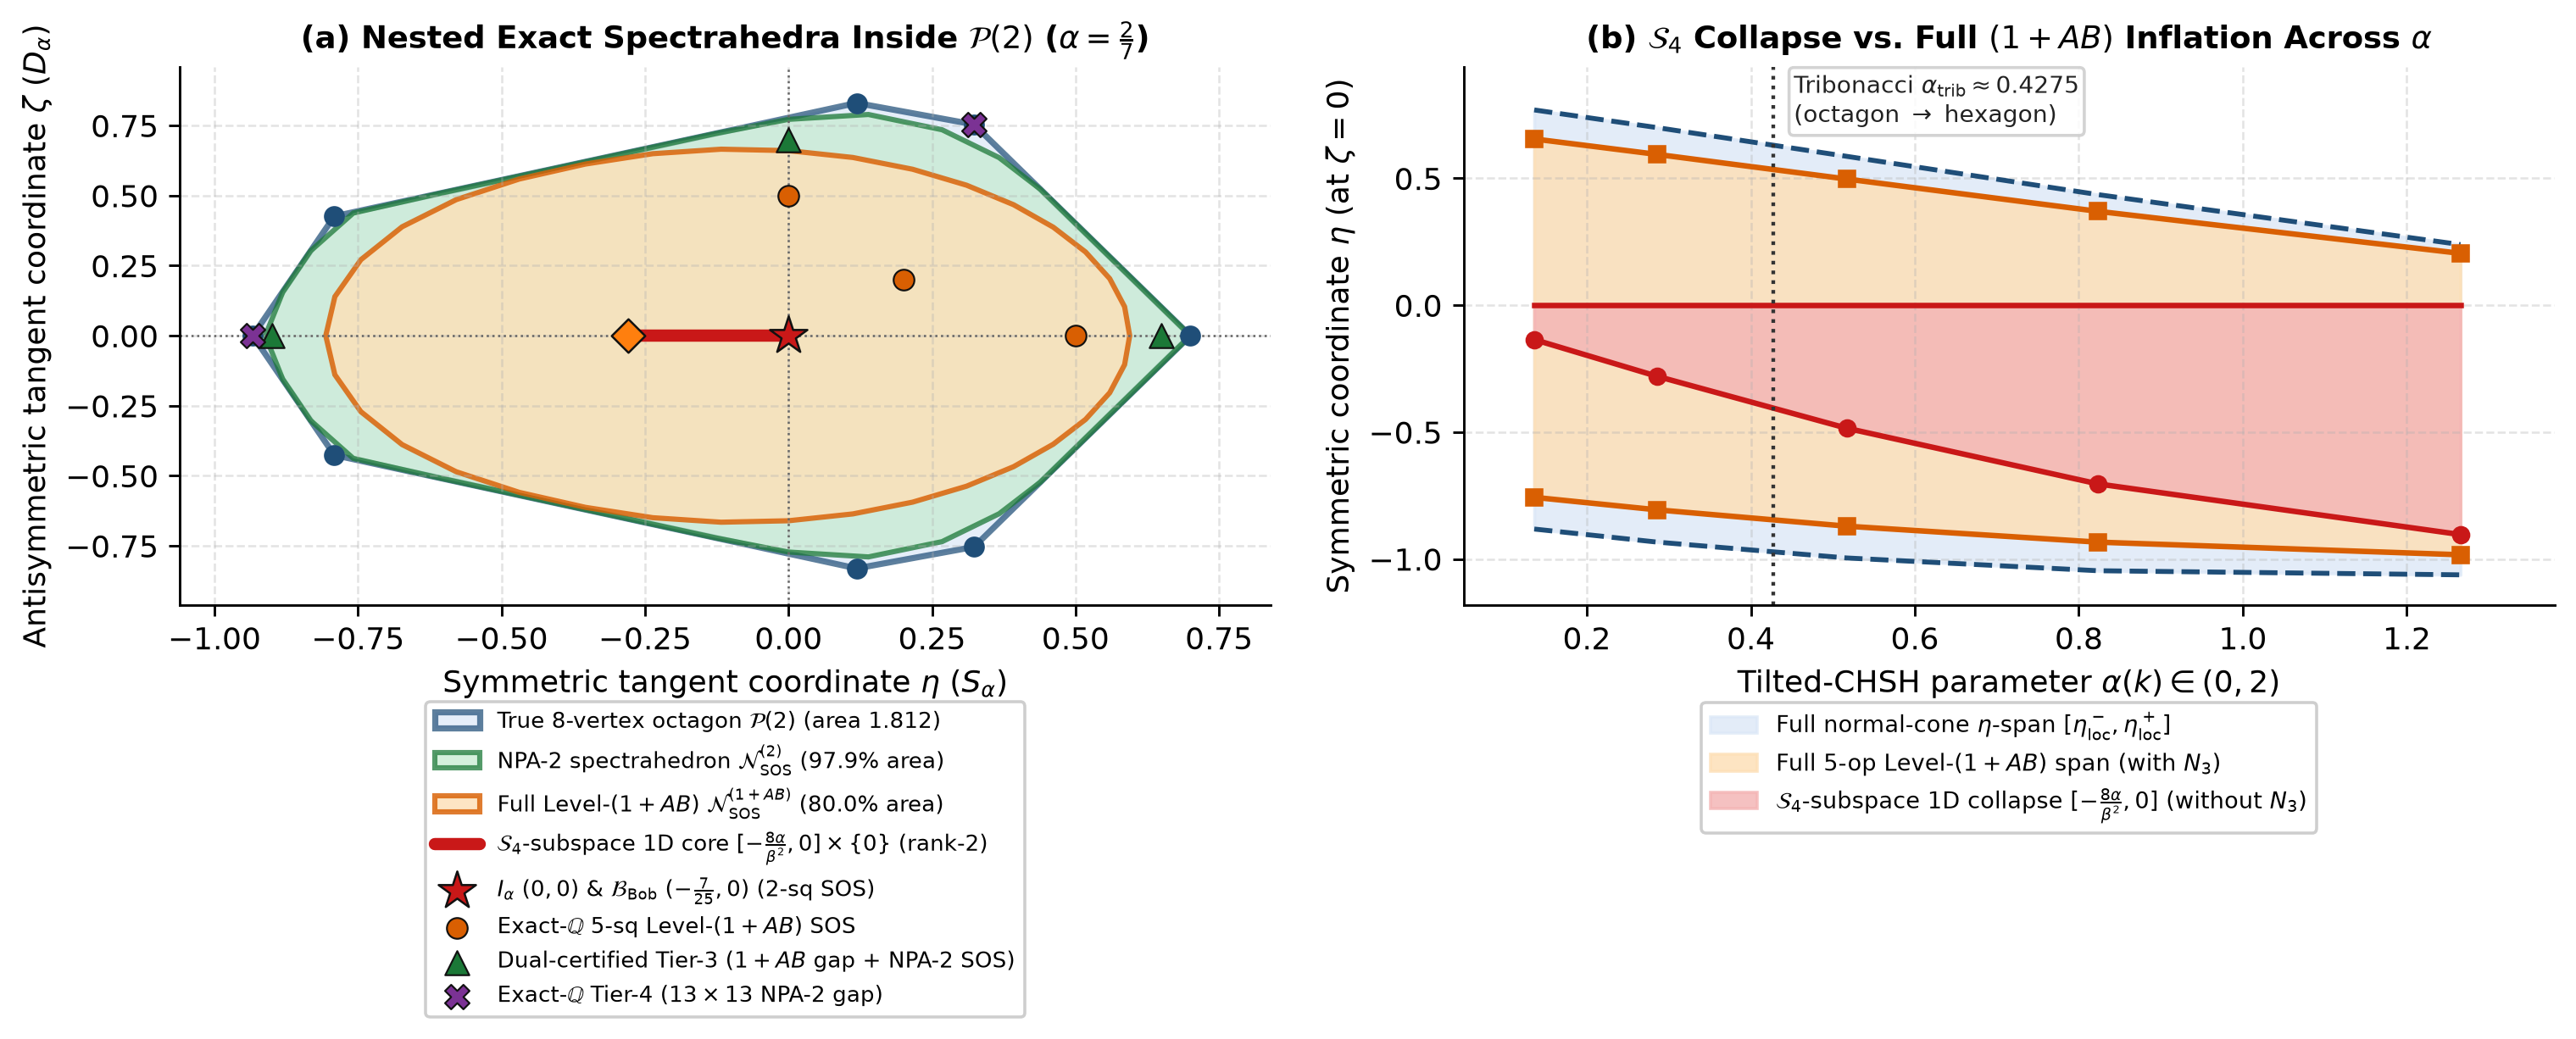
\includegraphics[width=\textwidth]{figures/fig1_normal_cone_collapse.png}
\caption{Nested spectrahedral geometry inside $\calN(p^*(k))$. \textbf{(a)}~At $k=2$ ($\alpha=2/7$), the exact 8-vertex octagon $\calP(2)$ (blue, area $1.812$) strictly encloses the curved NPA-2 spectrahedron $\mathcal{N}_{\mathrm{SOS}}^{(2)}$ (green, $97.9\%$ area), which strictly encloses the full 5-operator Level-$(1+AB)$ spectrahedron $\mathcal{N}_{\mathrm{SOS}}^{(1+AB)}$ (orange, $80.0\%$ area), containing the 1D $\calS_4$-subspace core $[-7/25, 0]\times\{0\}$ (red) from $I_\alpha$ to $\calB_{\mathrm{Bob}}$, overlaid with exact-$\QQ$ certified rays. \textbf{(b)}~Symmetric $\eta$-axis spans across $\alpha(k) \in (0,2)$ contrasting the 1D $\calS_4$ collapse with full Level-$(1+AB)$ inflation and marking the Tribonacci transition $\alpha_{\mathrm{trib}} \approx 0.4275$.}
\label{fig:spectrahedra}
\end{figure}

\subsection{Experiment 3: Nested Spectrahedral Phase Map and 4-Tier NPA Separation}

Experiment~3 maps both the 36-angle radial boundary contours of $\mathcal{N}_{\mathrm{SOS}}^{(1+AB)}(p^*(2))$ and $\mathcal{N}_{\mathrm{SOS}}^{(2)}(p^*(2))$ (Figure~\ref{fig:spectrahedra}(a)) and the exact Clarabel primal gaps $\Delta_{1+AB} = \beta_{\mathrm{NPA}}^{(1+AB)} - \beta_Q$ and $\Delta_2 = \beta_{\mathrm{NPA}}^{(2)} - \beta_Q$ across 18 probes (Figure~\ref{fig:npa-tiers}):
\begin{itemize}[leftmargin=1.5em,itemsep=1pt]
  \item \emph{Area stratification:} Out of the exact octagon area $1.81199$, the $\calS_4$ subspace covers $0.0\%$ (1D segment), full Level-$(1+AB)$ covers $1.45033$ ($80.0\%$), and NPA-2 covers $1.77359$ ($97.9\%$).
  \item \emph{Asymmetric apex behavior:} Notably, at the right apex $V_1 = (7/10, 0)$, Level-$(1+AB)$ exhibits a large gap $\Delta_{1+AB} = 1.941\times 10^{-2}$ (certified in $\QQ$ by \texttt{k2\_tier3\_vertex\_V1}) whereas NPA-2 becomes numerically tight ($\Delta_2 < 10^{-9}$). By contrast, the boundary point $(0, 7/9)$ ($\Delta_2 = 7.60 \times 10^{-4}$) and all seven remaining vertices $V_2, \dots, V_8$ exhibit strictly positive NPA-2 gaps up to $\Delta_2 = 1.659 \times 10^{-2}$ at $V_2, V_8$ and $7.628 \times 10^{-3}$ at the left apex $V_5 = (-14/15, 0)$.
\end{itemize}

\begin{figure}[t]
\centering
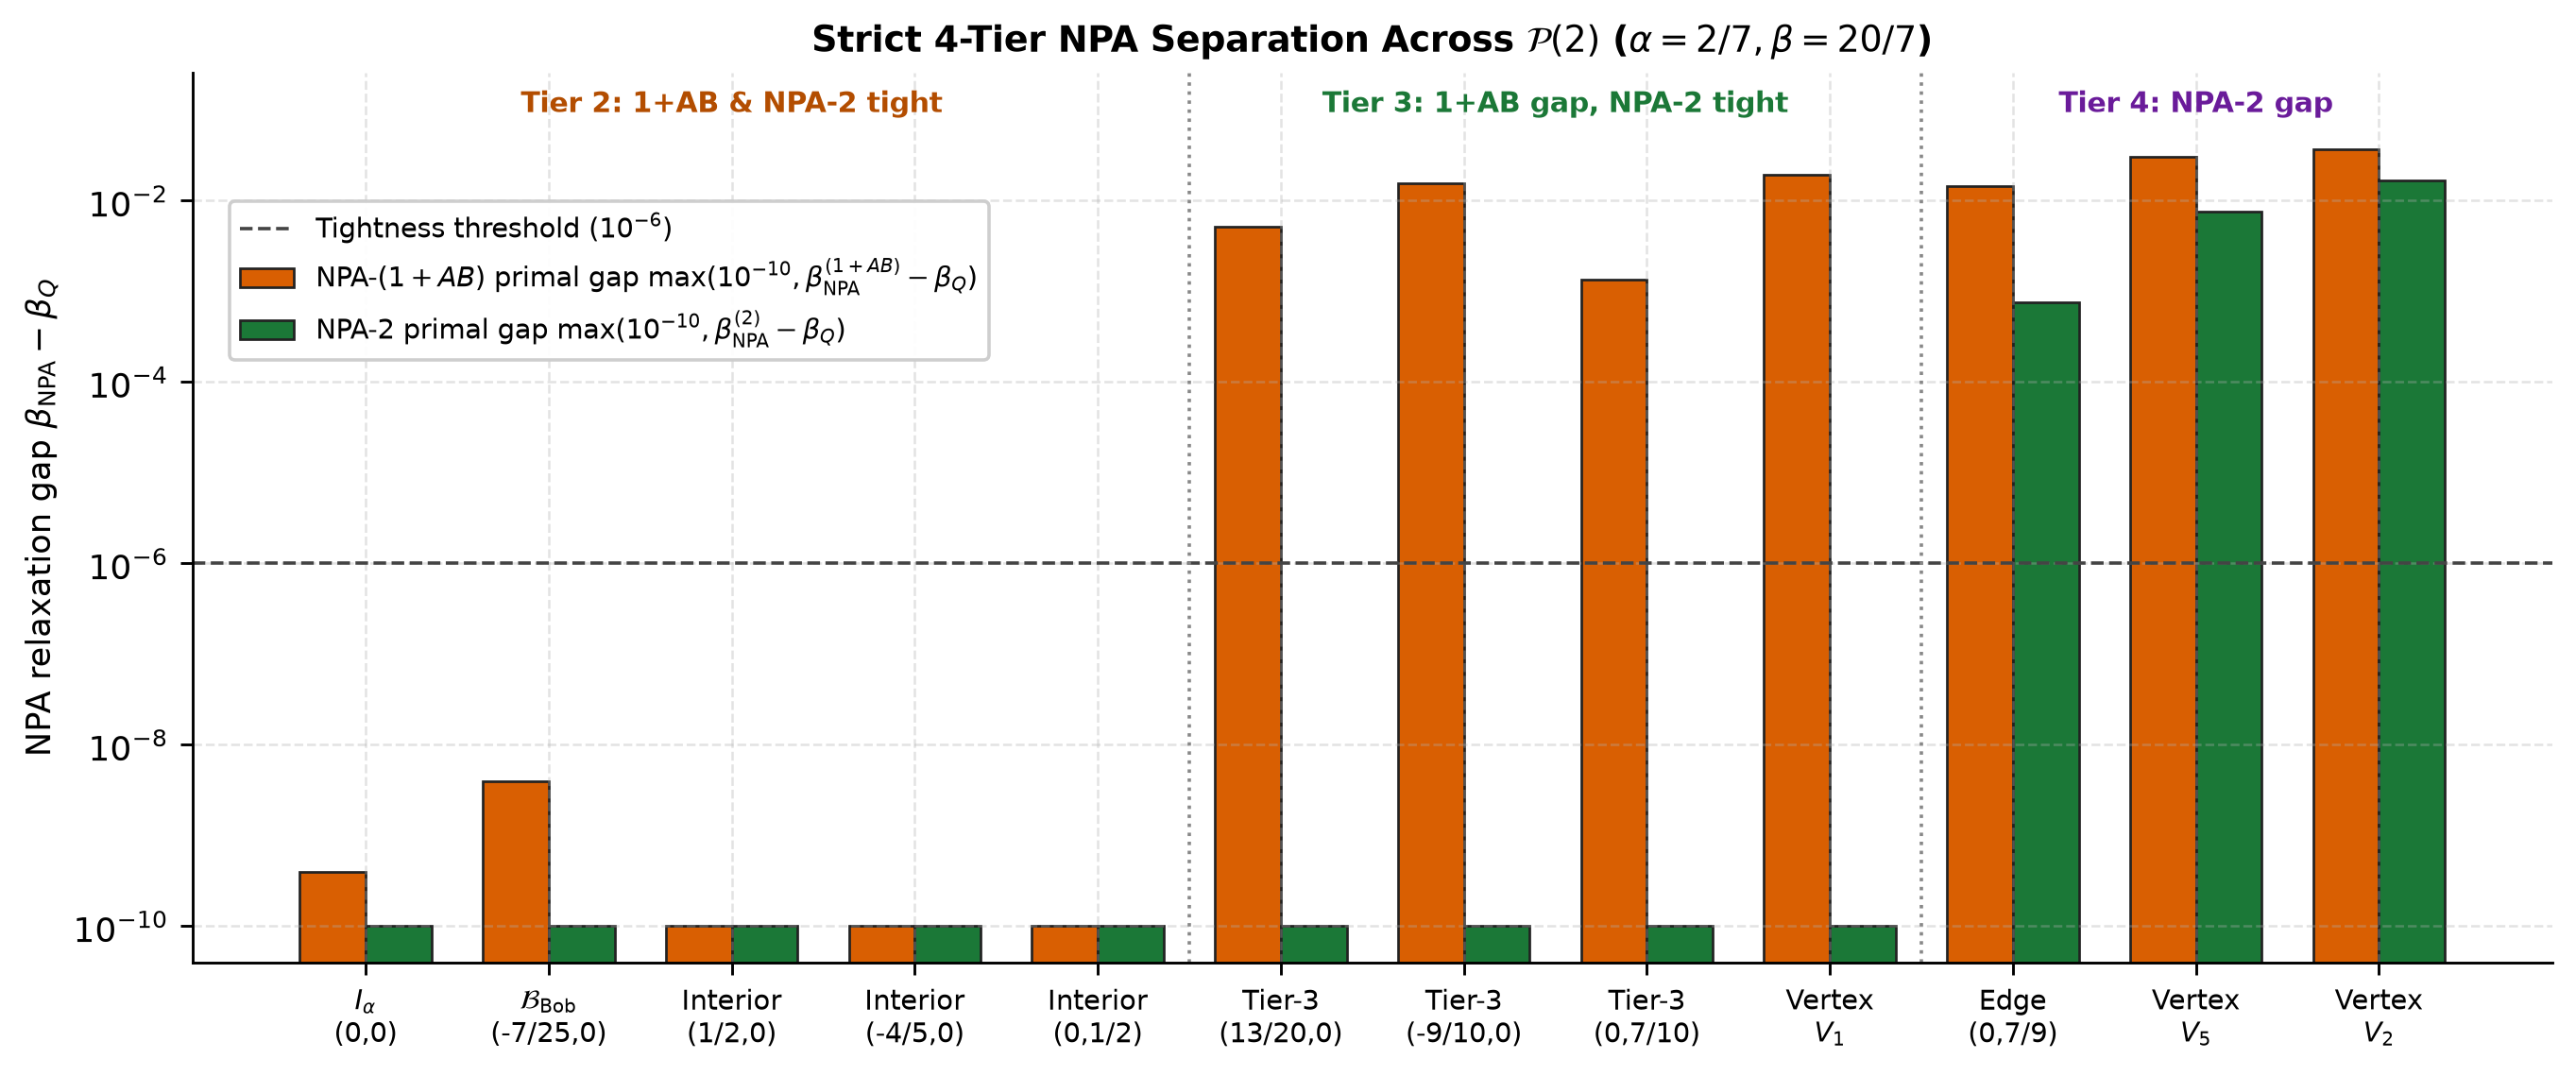
\includegraphics[width=\textwidth]{figures/fig2_npa_hierarchy_separation.png}
\caption{Experiment~3: Strict four-tier NPA primal relaxation gaps across $\calP(2)$ (\texttt{results/\allowbreak exp3\_npa\_hierarchy\_phase\_map.json}). Tier~2 interior points have zero gap at both $(1+AB)$ and NPA-2; Tier~3 points $(13/20,0)$, $(-9/10,0)$, $(0,7/10)$, and right apex $V_1$ show strict $(1+AB)$ gaps ($1.35\times 10^{-3}$--$1.94\times 10^{-2}$) resolved cleanly by NPA-2; Tier~4 edge $(0,7/9)$ and vertices $V_5, V_2$ retain strict gaps even at NPA-2.}
\label{fig:npa-tiers}
\end{figure}

\subsection{Experiment 4: Global White-Noise Visibility Landscape and 42-Attack Red-Team Audit}

Experiment~4 confirms Theorem~\ref{thm:visibility} independently across both LP solvers and exhaustive grids (Figure~\ref{fig:visibility}):
\begin{enumerate}[leftmargin=1.8em,itemsep=1pt]
  \item Across all five rational extreme points $k \in \{11/5, 2, 7/4, 3/2, 5/4\}$, independent HiGHS LP minimization of $\beta_{\mathrm{loc}}/\beta_Q$ over $\calP(k)$ recovers $(\eta_{\mathrm{opt}}, \zeta_{\mathrm{opt}}) = (0,0)$ and matches $v^*(\alpha) = (2+\alpha)/\beta$ to machine precision ($\max |\Delta v| = 3.33 \times 10^{-16}$).
  \item Across 739 interior and boundary grid points of $\calP(2)$, exact rational evaluation finds \textbf{zero violations} of $v(\eta,\zeta) \ge 4/5 = 0.80$, while the Bob-tilted endpoint $\calB_{\mathrm{Bob}}(\alpha)$ is strictly suboptimal across all $\alpha \in (0,2)$ (e.g., $29/35 \approx 0.8286$ vs.\ $4/5 = 0.8000$ at $k=2$).
\end{enumerate}

\begin{figure}[t]
\centering
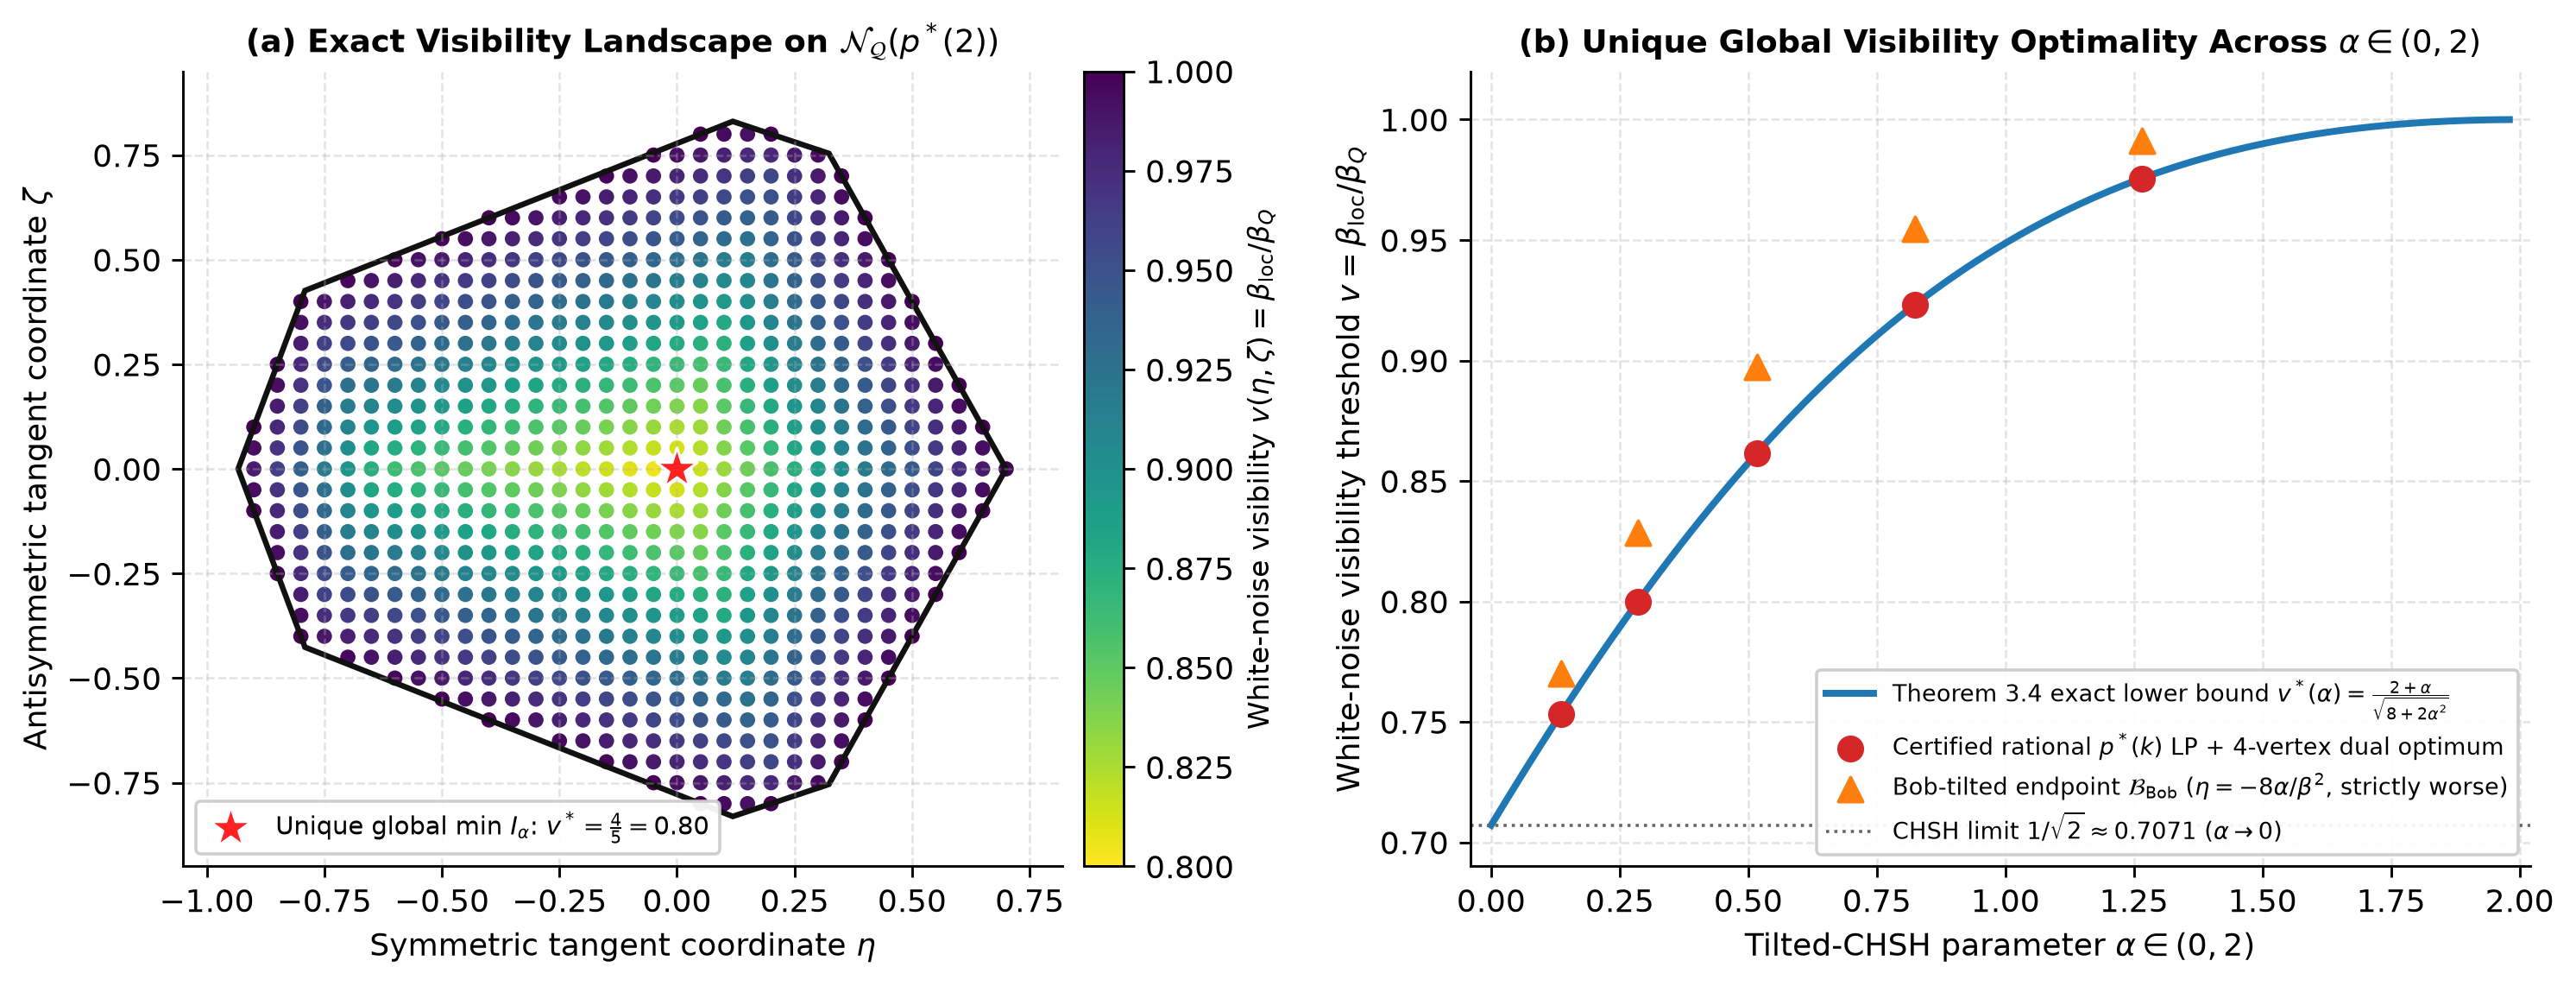
\includegraphics[width=\textwidth]{figures/fig3_visibility_optimality.png}
\caption{Experiment~4: Global white-noise visibility optimality of $I_\alpha$ across $\calN(p^*(k))$ (\texttt{results/\allowbreak exp4\_visibility\_optimality\_landscape.json}). \textbf{(a)}~Exact visibility threshold $v(\eta,\zeta) = \beta_{\mathrm{loc}}/\beta_Q$ across 739 grid points inside $\calP(2)$, attaining its unique global minimum $v^* = 4/5 = 0.80$ at $(0,0)$ with zero violations. \textbf{(b)}~Theorem~\ref{thm:visibility} lower bound $v^*(\alpha) = (2+\alpha)/\sqrt{8+2\alpha^2}$ versus HiGHS LP optima (red circles) and the strictly suboptimal Bob-tilted endpoint $\calB_{\mathrm{Bob}}$ (orange triangles).}
\label{fig:visibility}
\end{figure}

Finally, \texttt{tests/test\_suite.py} executes 4 verification suites covering all 9 annihilator norms on two-qubit realizations, the Tribonacci vertex-count transition, all 13 shipped certificates, and \textbf{42 live adversarial red-team attacks}: schema/key-set tampering, float/bool/Decimal/tuple injection, non-canonical rational strings (\texttt{"-0"}, \texttt{"2/1"}, \texttt{"4/14"}, \texttt{"+2"}, \texttt{"02"}, trailing newlines, Unicode digits), out-of-domain $k$, tampered $p^*$/$\beta_Q$/$\beta_{\mathrm{loc}}$, zero-square empty-polynomial injection, degree-2 word escape into Level-$(1+AB)$ SOS, degree-4 word escape into Level-2 SOS, negative/zero $LDL^\top$ pivots $D_i$, non-unit or upper-triangular $L$ corruption, broken NPA moment word-equivalence symmetry, tampered \texttt{npa\_gap}, forged universal visibility dual weights, and missing Tier-3 sub-payloads. All 42 attacks are deterministically rejected.

\section{Discussion and Outlook}
\label{sec:discussion}

Our findings clarify both the geometric richness and the exact semidefinite complexity of the Wu--Xie--Ramanathan normal cone $\calN(p^*)$~\cite{wu2026normalcone}.
First, the combinatorial boundary of $\calP(k)$ undergoes an unexpected algebraic transition from an octagon to a hexagon precisely at the Tribonacci constant $k_{\mathrm{trib}} \approx 1.839287$.
Second, the exact annihilator $N_3$ plays a dramatic structural role at NPA Level-$(1+AB)$: omitting $N_3$ collapses the entire SOS cone to the 1D rank-2 segment $\conv\{I_\alpha, \calB_{\mathrm{Bob}}(\alpha)\}$, whereas including all five Level-$(1+AB)$ annihilators inflates it to $80.0\%$ of the polygon area, leaving a $17.9\%$ collar certified at NPA-2 and a $2.1\%$ outer corner region around extreme vertices $V_2, \dots, V_8$ requiring NPA-3 or higher.
Third, our four-vertex LP dual theorem proves that no normal-cone deformation can improve isotropic white-noise visibility over $I_\alpha$; hence the practical device-independent gains of exploring $\calN(p^*)$~\cite{wu2026normalcone} arise specifically for asymmetric operational metrics such as one-sided randomness certification~\cite{wooltorton2022tight}, directional noise models, or marginal-free designs like $\calB_{\mathrm{Bob}}$.

\section*{Reproducibility and Artifact Verification}
The complete codebase, Lean~4 formalization, 13 exact-$\QQ$ certificates, experimental outputs, figures, and SHA-256 manifest are publicly archived under the MIT License at \url{https://github.com/lluiseriksson/normal-cone-sos-hierarchy}.
Running \texttt{python scripts/verify\_all.py} independently replays: (1) the Lean~4 \texttt{v4.35.0} build and axiom audit (20/20 theorems, 0 warnings, 0 \texttt{sorry}, 0 \texttt{Classical.choice}); (2) zero-float exact-$\QQ$ verification of all 13 certificates; (3) the full \texttt{pytest} suite including all 42 live adversarial attacks; and (4) SHA-256 integrity checks across all 36 tracked repository artifacts.

\bibliographystyle{unsrt}
\bibliography{references}

\end{document}
